\documentclass{../FYPFast/FastFyp}

\usepackage[T1]{fontenc}
\usepackage[utf8]{inputenc}
\usepackage{booktabs,longtable,tabularx,array,multirow}
\usepackage{enumitem,float,adjustbox,pdflscape}
\usepackage{xcolor}
\usepackage{tikz}
\usetikzlibrary{arrows.meta,positioning,shapes.geometric,fit,backgrounds,calc,matrix}
\definecolor{manzilblue}{HTML}{184E77}
\definecolor{manzilgreen}{HTML}{2A9D8F}
\definecolor{manzilamber}{HTML}{E9C46A}
\definecolor{manzilred}{HTML}{D1495B}
\definecolor{manzilgray}{HTML}{F3F5F7}
\hypersetup{pdftitle={Manzil: Intelligent Traffic and Emergency Routing},pdfauthor={Muhammad Ali Mahoon, Muzammil Ahmed Bhatti, Mohammad Ibrahim Salman}}
\setlength{\headheight}{15pt}
\setcounter{tocdepth}{2}
\newcolumntype{Y}{>{\raggedright\arraybackslash}X}
\newcommand{\status}[1]{\textit{#1}}
\newcommand{\fr}[1]{\textbf{FR-#1}}
\newcommand{\nfr}[1]{\textbf{NFR-#1}}
\newcommand{\todo}[1]{\fcolorbox{manzilred}{manzilgray}{\parbox{0.92\linewidth}{\textbf{TODO:} #1}}}

\begin{document}
\newcommand{\supervisor}{Miss Umm-e-Ammarah}
\newcommand{\university}{National University of Computer and Emerging Sciences, Lahore}
\newcommand{\fyptitle}{Manzil: Intelligent Traffic \& Emergency Routing}
\newcommand{\reporttype}{Deliverable 2 Report}
\date{7 October 2026}
\renewcommand{\contentsname}{Table of Contents}

\makeatletter
\begin{titlepage}
  
\includegraphics[width=0.19\linewidth]{../FYPFast/Figures/nulogo.png}\hfill
  
\includegraphics[width=0.19\linewidth]{../FYPFast/Figures/fast.png}
  \begin{center}
    \vspace{1.0cm}
    {\large\bfseries \university}\par
    \vspace{1.2cm}
    
\includegraphics[width=0.34\linewidth]{../FYPFast/Figures/fastlogo.png}\par
    \vspace{1.4cm}
    {\Huge\bfseries \fyptitle\par}
    \vspace{0.7cm}
    {\Large \reporttype\par}
    \vspace{0.4cm}
    {\large Project/Group ID: F26-104\par}
    \vspace{1.1cm}
    \begin{tabular}{ll}
      Muhammad Ali Mahoon & 23L-0531\\
      Muzammil Ahmed Bhatti & 23L-0688\\
      Mohammad Ibrahim Salman & 23L-0723
    \end{tabular}
    \vspace{0.8cm}

    {Supervisor: \supervisor\par}
    \vfill
    {Department of Computer Science\par}
    {Final Year Project\par}
    {\large \@date\par}
  \end{center}
\end{titlepage}
\makeatother

\frontmatter
\cleardoublepage
\thispagestyle{empty}
\section*{Anti-Plagiarism Declaration}
We declare that this report, entitled \emph{\fyptitle}, is the original work of the listed authors. Material derived from other work has been identified and cited. No part has been reproduced in a manner that constitutes plagiarism. We accept responsibility for any violation established under the University's academic-integrity policy.

\vspace{1cm}
\begin{tabularx}{\textwidth}{Y Y}
Date: \rule{4cm}{0.4pt} & Muhammad Ali Mahoon: \rule{4cm}{0.4pt}\\[1.2cm]
& Muzammil Ahmed Bhatti: \rule{4cm}{0.4pt}\\[1.2cm]
& Mohammad Ibrahim Salman: \rule{4cm}{0.4pt}
\end{tabularx}

\vfill
\hrule
\section*{Authors' Declaration}
We declare that the work presented in this Deliverable 2 report is our own project work and has not been submitted previously, in whole or in part, to another institution for an academic award. This document describes a proposed system and planned evaluation; it does not present unperformed experiments as completed results.

\cleardoublepage
\section*{Abstract}
Manzil is a simulation-based research and development prototype for adaptive urban traffic control and emergency routing. It combines video-based vehicle detection and tracking, traffic-state estimation, comparative signal-control policies, congestion-aware ambulance routing, and a moving green corridor within a SUMO test environment. A React dashboard and FastAPI services are proposed to expose system state and experimental records. This report specifies the requirements, research method, architecture, and controlled evaluation protocol; implementation and measured results remain subsequent project work.

\cleardoublepage
\section*{Executive Summary}
Urban road demand changes over time and between approaches, whereas a fixed timing plan cannot respond to every short-term imbalance. Emergency vehicles face a related but stricter problem: a geographically short route can still be slow when queues, signal delay, or an incident obstruct the path. Manzil studies these two problems in one controlled prototype. The system is intended to compare fixed-time, rule-based adaptive, and reinforcement-learning signal control, then determine the contribution of dynamic routing and a moving green corridor to ambulance travel while measuring the disruption imposed on ordinary traffic.

The project deliberately separates two evidence paths. Recorded traffic video is used to study whether a detector and multi-object tracker can produce observable counts, speeds, and queue proxies. SUMO and TraCI provide exact, repeatable network state for controller and routing experiments. These paths share a versioned traffic-state contract, but this report does not claim that arbitrary camera footage reconstructs a complete road network. Camera calibration, lane mapping, observation freshness, and uncertainty are explicit constraints.

The proposed system uses a React dashboard, FastAPI application services, a background perception worker, a SUMO/TraCI adapter, controller and routing services, and persistent experimental records. PostgreSQL is a proposed persistence choice rather than a confirmed implementation fact. A selected, manageable urban network is to be imported from OpenStreetMap and cleaned in SUMO NetEdit, with a synthetic grid retained as a fallback. The core emergency case contains one active ambulance. Dynamic edge costs combine estimated travel time, queue and signal delay without treating distance alone as the objective. Priority is activated only for the next relevant intersections, uses safe clearance transitions, detects passage, and then restores normal operation.

Evaluation is planned as matched, repeated simulation runs under light, medium, and heavy demand. Normal traffic experiments compare the three controllers using travel time, waiting time, queue length, throughput, and starvation checks. Emergency experiments compare an unassisted reference, congestion-aware routing, and routing with corridor control using ambulance travel time and stops together with normal-traffic delay and recovery time. Training and tuning scenarios will be separated from held-out evaluation scenarios, and all configurations, random seeds, software versions, and failures will be retained. No performance values are reported at this Deliverable 2 stage.

This report covers the project vision, a critical review of relevant research, software requirements, the proposed research method, and high- and low-level design. Its main contribution at this stage is a traceable and reproducible specification for investigating an integrated traffic-control and emergency-priority approach without overstating implementation maturity or real-world deployability.

\pagestyle{fancy}
\tableofcontents
\cleardoublepage
\listoffigures
\addcontentsline{toc}{chapter}{List of Figures}
\cleardoublepage
\listoftables
\addcontentsline{toc}{chapter}{List of Tables}

\mainmatter
\chapter{Introduction}
\label{ch:introduction}

Urban traffic control is a networked decision problem. Demand can change by approach, queue spillback at one junction can obstruct another, and a timing plan that is adequate in one period may waste capacity in another. Emergency travel adds a stricter timing objective. An ambulance does not benefit merely from a short geometric path if that path contains slow links, long queues, or signals that repeatedly stop it. These observations motivate Manzil, a research and development prototype that studies traffic perception, adaptive signal control, congestion-aware emergency routing, and coordinated signal priority in one simulation-based environment.

Manzil is not presented as a deployable municipal controller. It is a controlled experimental platform based on the microscopic traffic simulator SUMO and its TraCI interface \cite{lopez2018sumo,sumodocs}. The platform is intended to make policies repeatable, observable, and comparable before any real-world actuation is considered. Recorded video supplies a second, deliberately bounded input mode for studying whether vehicle detection and tracking can produce useful traffic indicators. The simulator remains the authoritative source of network state in routing and signal-control experiments.

\section{Purpose of this Document}

This Deliverable 2 report translates the approved proposal into a traceable research and software design. It defines the questions to be investigated, reviews the evidence behind major design choices, specifies externally visible requirements, and describes the methodology and architecture needed to conduct fair experiments. It also records the distinction between confirmed project scope, proposed technical choices, and future implementation work.

The report does not claim experimental improvements, real-time performance, model accuracy, or deployment readiness. At the proposal stage the problem definition, major functions, and conceptual architecture were established; dataset preparation, implementation, tuning, and evaluation were still planned work. The methodology therefore defines how later claims must be produced rather than anticipating their outcome.

\section{Intended Audience}

The primary audience is the FAST--NUCES FYP supervisor and evaluation panel. They require enough detail to judge research relevance, software scope, feasibility, and the validity of the proposed evaluation. The report is also written for the student implementation team, who should be able to derive interfaces, experiment configurations, and acceptance checks from it. A secondary audience consists of traffic-domain and emergency-service stakeholders who may assess the assumptions and limitations, although those stakeholders are not treated as current project clients.

\section{Project Status and Evidence Boundaries}
\label{sec:status}

Table \ref{tab:status} prevents proposed components from being read as completed ones. A choice is described as ``proposed'' where the repository contains a design decision but no implementation artifact or measured evidence. This convention is used throughout the report.

\begin{table}[H]
\centering
\caption{Project status at Deliverable 2}
\label{tab:status}
\begin{tabularx}{\textwidth}{p{0.25\textwidth}YY}
\toprule
\textbf{Area} & \textbf{Confirmed evidence} & \textbf{Not yet evidenced}\\
\midrule
Problem and scope & Approved proposal, objectives, exclusions, and simulation basis & Field deployment or agency integration\\
Architecture & Conceptual React/FastAPI/SUMO and perception decomposition & Deployed services and measured capacity\\
Traffic control & Fixed, rule-adaptive, and RL comparison plan & Final RL policy and comparative results\\
Emergency operation & Dynamic route and moving-corridor design & Validated timing parameters and achieved savings\\
Perception & YOLO-based detector and tracker direction & Final checkpoint, annotated split, and measured accuracy\\
Data persistence & Experiment records and candidate entities & Confirmed database engine and schema migrations\\
\bottomrule
\end{tabularx}
\end{table}

\section{Definitions, Acronyms, and Abbreviations}

\begin{longtable}{p{0.19\textwidth}p{0.72\textwidth}}
\caption{Key terminology}\label{tab:terms}\\
\toprule
\textbf{Term} & \textbf{Definition in this report}\\
\midrule\endfirsthead
\toprule
\textbf{Term} & \textbf{Definition in this report}\\
\midrule\endhead
A* & A shortest-path search that ranks candidates using accumulated cost plus an admissible lower-bound heuristic \cite{hart1968astar}.\\
API & Application Programming Interface.\\
CV & Computer vision; here, processing traffic video into observable vehicle-level and aggregate indicators.\\
Green corridor & A sequence of bounded, moving signal-priority interventions ahead of an ambulance; not permanent green on the whole route.\\
MOT & Multi-object tracking, which associates detections into identities across frames.\\
Queue proxy & An operational estimate based on tracked, slow or stationary vehicles in a defined lane region; not a direct physical queue measurement unless calibrated.\\
RL & Reinforcement learning, in which a policy is optimized using state, actions, and cumulative reward.\\
Signal preemption & Interruption or modification of normal signal operation to serve an emergency request, including transition and recovery.\\
SUMO & Simulation of Urban MObility, a microscopic road-traffic simulator.\\
TraCI & Traffic Control Interface, used by an external process to read and change a running SUMO simulation.\\
Traffic-state contract & Versioned representation of approach observations, signal state, source mode, timestamps, units, confidence, and validity.\\
Throughput & Vehicles completing a defined movement or leaving a measured network region per unit time.\\
Waiting time & Time accumulated under the explicitly configured low-speed threshold; the exact SUMO definition and threshold will be recorded with each experiment.\\
\bottomrule
\end{longtable}

\section{Report Organization}

Chapter \ref{ch:vision} defines the problem, objectives, boundaries, stakeholders, constraints, and research questions. Chapter \ref{ch:literature} critically reviews perception, traffic-control, routing, and emergency-priority research. Chapter \ref{ch:srs} specifies functional and quality requirements, use cases, wireframes, data, risk, and traceability. Chapter \ref{ch:method} defines the proposed pipelines, algorithms, experimental protocol, metrics, and validity controls. Chapter \ref{ch:design} presents the component architecture, domain model, interactions, corridor lifecycle, contracts, concurrency model, and engineering policies.

\section{Conclusion}

Manzil is framed as a reproducible investigation of interacting traffic decisions rather than as a collection of unrelated AI features. The remainder of the report maintains a strict boundary between planned methods and completed evidence, which is essential for evaluating Deliverable 2 on the quality of its design.


\chapter{Project Vision}
\label{ch:vision}

This chapter converts the broad motivation into a bounded project vision. It identifies the decisions Manzil will make, the evidence needed to judge those decisions, and the conditions under which conclusions will remain limited to simulation and selected video.

\section{Problem Domain Overview}

Traffic-signal control allocates time among incompatible movements. Fixed plans are understandable and easy to reproduce, but cannot react to short-term imbalance. Adaptive control can use measured demand, yet an apparently efficient policy can be unfair if a lightly loaded approach waits indefinitely. Network coordination complicates the problem because an action at one intersection changes arrivals at downstream intersections.

Emergency routing operates on the same network but has a different objective. A route is useful only when its costs reflect current travel time and intersection delay. Signal priority can reduce stops, but careless preemption can create unsafe phase changes or long recovery queues. The project therefore treats route selection, priority activation, passage detection, and recovery as one lifecycle while retaining separate measurements for the ambulance and ordinary traffic.

\begin{figure}[H]
\centering
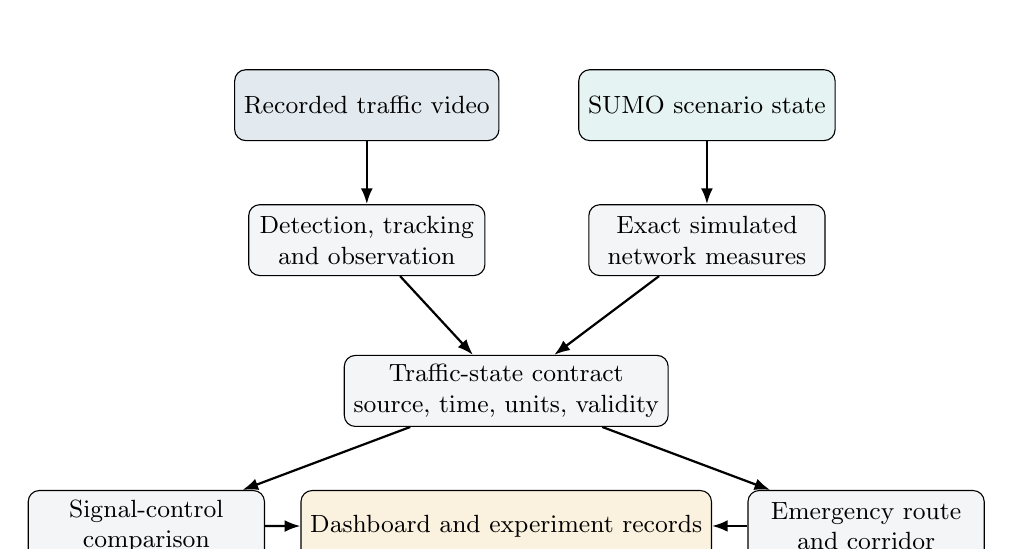
\begin{tikzpicture}[font=\small,node distance=8mm and 10mm,
box/.style={draw,rounded corners,fill=manzilgray,minimum width=3.0cm,minimum height=0.9cm,align=center},
arr/.style={-{Latex[length=2mm]},thick}]
\node[box,fill=manzilblue!12] (video) {Recorded traffic video};
\node[box,right=of video,fill=manzilgreen!12] (sim) {SUMO scenario state};
\node[box,below=of video] (per) {Detection, tracking\\and observation};
\node[box,below=of sim] (truth) {Exact simulated\\network measures};
\node[box,below right=10mm and -18mm of per,minimum width=4cm] (contract) {Traffic-state contract\\source, time, units, validity};
\node[box,below left=of contract] (ctrl) {Signal-control\\comparison};
\node[box,below right=of contract] (em) {Emergency route\\and corridor};
\node[box,below=of contract,fill=manzilamber!22] (dash) {Dashboard and experiment records};
\draw[arr] (video)--(per); \draw[arr] (sim)--(truth);
\draw[arr] (per)--(contract); \draw[arr] (truth)--(contract);
\draw[arr] (contract)--(ctrl); \draw[arr] (contract)--(em);
\draw[arr] (ctrl)--(dash); \draw[arr] (em)--(dash);
\end{tikzpicture}
\caption{Manzil project context and the separation of evidence paths}
\label{fig:context}
\end{figure}

Figure \ref{fig:context} shows the central scope decision. Video observations may be evaluated against annotations, while SUMO state drives repeatable control experiments. Both can populate a common contract, but a measurement from one source is never silently treated as ground truth from the other.

\section{Problem Statement}

The project addresses the absence, within the selected prototype setting, of a reproducible way to compare traffic-signal strategies and to quantify the combined effect of congestion-aware ambulance routing and coordinated signal priority. The problem is to design a system that observes or simulates traffic state, makes bounded control and routing decisions, records their causes and outcomes, and supports fair comparison without claiming that simulation results transfer directly to a deployed city.

\section{Problem Elaboration}

Five linked sub-problems must be controlled. First, detections must be associated over time so that frame-level boxes can become counts, trajectories, and lane-region observations. Second, normal signal control requires fixed and adaptive baselines before RL is meaningful. Third, route costs must use consistent units and must not count congestion twice. Fourth, the corridor must anticipate an ambulance without holding unnecessary intersections green. Fifth, all comparisons must use matched demand, seeds, and configurations.

An error can cross module boundaries. A stale observation may alter an edge cost; a route change may invalidate planned signal priority; a prolonged priority phase may improve ambulance time while worsening ordinary traffic; and an uncontrolled simulation clock may allow different services to act on different steps. The vision therefore includes explicit freshness, ownership, fallback, and audit requirements.

\section{Research Questions}

\begin{description}[style=nextline,leftmargin=1.7cm]
\item[RQ1] With declared video sources and annotations, how accurately and consistently can the proposed detector-tracker pipeline estimate observable vehicle counts and queue-related indicators?
\item[RQ2] Under matched SUMO demand scenarios, how do fixed-time, rule-based adaptive, and a selected RL controller differ in waiting time, queue length, travel time, throughput, and approach fairness?
\item[RQ3] Holding signal control constant, what change in ambulance travel time, stops, and route stability is attributable to dynamic congestion-aware routing?
\item[RQ4] Holding routing logic constant, what additional emergency benefit and ordinary-traffic disruption result from the moving green corridor?
\item[RQ5] How sensitive are the conclusions to demand level, incident placement, random seed, and observation uncertainty?
\end{description}

These questions avoid a single vague claim of ``better traffic.'' Each comparison names a controlled factor and paired outcome measures.

\section{Goals and Objectives}

The goal is to develop and evaluate a simulation-based intelligent traffic-management prototype that supports normal traffic control and a single emergency mission. The measurable objectives are:

\begin{enumerate}[label=O\arabic*.]
\item Define and implement a versioned traffic-state representation shared by perception, simulation, control, routing, and visualization.
\item Evaluate a pretrained vehicle detector with multi-object tracking on held-out, source-separated traffic-video segments.
\item Construct a manageable multi-intersection SUMO network and repeatable demand scenarios.
\item Implement fixed-time and reproducible rule-adaptive controllers, followed by one feasible RL controller.
\item Compute valid ambulance routes using time-based dynamic edge costs and bounded rerouting.
\item Coordinate safe, moving signal priority and restore normal control after passage or cancellation.
\item Provide a React dashboard and FastAPI service boundary for scenario control, monitoring, and experiment comparison.
\item Record configurations and outcomes so each reported run can be reproduced and audited.
\end{enumerate}

\section{Project Scope}

\begin{table}[H]
\centering
\caption{Scope boundaries}
\label{tab:scope}
\begin{tabularx}{\textwidth}{YY}
\toprule
\textbf{In scope} & \textbf{Outside the current scope}\\
\midrule
Recorded-video vehicle detection, tracking, counts, and queue proxies & Live government CCTV integration or citywide camera calibration\\
Selected multi-intersection SUMO network and synthetic demand & All of Lahore or safety-certified field deployment\\
Fixed, rule-adaptive, and one RL controller & Replacing real traffic-controller firmware\\
Single active ambulance with dynamic routing and moving priority & Multiple competing emergency fleets as a core case\\
Simulated closure or incident as a routing trigger & Visual accident classification or traffic forecasting\\
React dashboard, FastAPI services, and experiment records & Native mobile application, enforcement, facial or number-plate recognition\\
OpenStreetMap import with manual cleanup where feasible & A guarantee that map attributes are complete or current\\
\bottomrule
\end{tabularx}
\end{table}

\section{Sustainable Development Goals}

Manzil aligns principally with United Nations Sustainable Development Goal 11, which concerns inclusive, safe, resilient, and sustainable cities \cite{un2025sdg}. The project investigates more efficient use of existing intersection capacity and more timely emergency movement, but it does not claim city-level impact from a simulator. A secondary connection exists with health outcomes because ambulance delay can matter, although the project neither measures clinical outcomes nor models medical priority.

\section{Constraints and Assumptions}

The main constraints are a semester-scale implementation window, limited access to local calibrated traffic data, camera occlusion and perspective, the simulation-to-reality gap, and finite training hardware. The selected network must therefore remain small enough for repeated trials. A real urban extract is preferred, but a controlled grid is an acceptable fallback if map signal logic is incomplete.

The core experiments assume one active ambulance, valid origin and destination edges, controlled traffic generation, and no direct actuation of public infrastructure. Video-derived queue length is an observable proxy unless the scene is calibrated. PostgreSQL, the precise tracker, the RL algorithm, and computing hardware remain proposed choices until implementation evidence confirms them.

\section{Business and Practical Opportunity}

The prototype's practical value is as a decision-support and experimentation environment. It can demonstrate how policies react to repeatable congestion and emergency scenarios, help compare controller designs, and expose the cost imposed on non-priority traffic. Any commercial or public-sector opportunity would require validated local data, authority approval, hardware integration, cybersecurity assessment, safety engineering, and field trials. No partnership, deployment commitment, or revenue expectation is assumed.

\section{Stakeholders and User Characteristics}

\begin{table}[H]
\centering
\caption{Stakeholder summary}
\label{tab:stakeholders}
\begin{tabularx}{\textwidth}{p{0.24\textwidth}YY}
\toprule
\textbf{Stakeholder} & \textbf{Interest} & \textbf{Expected interaction}\\
\midrule
Student research team & Correct implementation and defensible experiments & Configure, run, diagnose, export, and compare experiments\\
Supervisor and evaluators & Scope, rigor, traceability, and evidence quality & Review report, configurations, demonstrations, and results\\
Prototype operator & Clear scenario and emergency controls & Use the dashboard; inspect warnings and system state\\
Prospective traffic authority & Safety, reliability, network impact, auditability & Future consultation only; no current operational role\\
Prospective emergency service & Travel-time benefit and predictable priority behavior & Future requirements input only\\
Road users & Fairness and limited disruption & Indirect beneficiaries or affected parties in simulated evaluation\\
\bottomrule
\end{tabularx}
\end{table}

\section{Success Criteria}

Deliverable success is not defined by a visually impressive ambulance alone. The research prototype should execute matched scenarios without hidden configuration changes, record all interventions, reject invalid routes and stale inputs, and report both benefits and side effects. A conclusion is considered supported only when it is tied to a named scenario set, repeated seeds, variability, and an unchanged measurement definition.

\section{Conclusion}

The vision is deliberately narrower than real traffic management: a controlled, auditable prototype with one core emergency case and explicit evidence boundaries. These boundaries shape the literature review and prevent later design choices from silently expanding the approved scope.


\chapter{Literature Review and Related Work}
\label{ch:literature}

This chapter examines the research needed to justify Manzil's design rather than treating the use of familiar tools as a contribution. The review is organized around five decisions: how traffic is observed, how normal signals are controlled, how learned policies are evaluated, how emergency routes are selected, and how signal priority is activated and recovered. Each study is considered in its original data or simulation setting because reported values from incompatible benchmarks cannot be treated as a common comparison. The discussion identifies the method, evidence, limitations, and direct implication for a Manzil design choice. Research papers are distinguished from official software documentation, which is used to establish interface capabilities but is not counted toward the study requirement. The purpose is not to assemble every publication on intelligent transportation. It is to establish whether the proposed components are technically defensible, which assumptions must be recorded, and where a controlled undergraduate experiment can add useful evidence. The final synthesis consequently states a precise integration question instead of claiming that the use of YOLO, reinforcement learning, or shortest-path search is itself novel.

\section{Review Method and Terminology}

The approved proposal supplied the initial bibliography, after which each retained study was checked against a publisher page, proceedings record, DOI, or official open-access paper. Selection required direct relevance to vehicle detection and tracking, traffic-state estimation, signal control, simulation, graph routing, or emergency preemption. The review also applies consistent terminology. Detection refers to locating and classifying vehicles within one frame, while tracking refers to associating those observations through time. A detector therefore cannot produce reliable passage counts by itself. Signal priority describes preferential treatment that may remain within normal timing constraints, whereas preemption may interrupt normal operation for an emergency request. Manzil uses the term moving green corridor for a coordinated sequence of bounded interventions ahead of the ambulance, not for a permanently green route. These distinctions affect the interpretation of prior results and the design of the proposed experiment. A paper reporting benchmark detection accuracy does not establish a calibrated queue estimate, and a study of isolated preemption does not automatically validate network-level routing. The following sections preserve those boundaries when relating the literature to Manzil.

\section{Vision-Based Traffic Observation}

\subsection{One-Stage Object Detection}

Redmon et al. formulated YOLO as a single network that predicts bounding boxes and class probabilities from an image in one evaluation \cite{redmon2016yolo}. The study established the feasibility of real-time one-stage detection and reported a strong speed advantage, while also identifying localization error as a relative weakness. The design is relevant to Manzil because a compact inference path is practical for recorded traffic video and may later support a live demonstration on available hardware. The evidence does not establish accuracy for every vehicle class, road layout, camera height, weather condition, or Lahore traffic scene. A selected pretrained checkpoint must therefore be evaluated on the project's own held-out sequences, and confidence or intersection-over-union thresholds cannot be copied from an unrelated benchmark. Frame-level boxes also do not provide stable counts by themselves. The same vehicle may be detected in many frames, an occluded vehicle may disappear temporarily, and perspective changes apparent size across the image. Manzil consequently treats one-stage detection as the first part of a measurement pipeline that also requires tracking, road-region assignment, temporal aggregation, and explicit uncertainty.

\subsection{Multi-Object Association}

Wojke et al. extended a simple online tracker with a learned appearance metric to improve association through longer occlusions \cite{wojke2017deepsort}. Appearance information can reduce identity switches, but it adds a feature-extraction model, processing cost, and sensitivity to domain differences. ByteTrack follows a different strategy by associating high-confidence detections first and then attempting to recover true objects from lower-confidence boxes rather than discarding them \cite{zhang2022bytetrack}. The authors evaluated it across several tracking benchmarks and reported strong accuracy with real-time throughput on their stated hardware. This approach is relevant to traffic video because occlusion and motion blur often reduce detection confidence. Neither benchmark establishes Manzil's processing speed, lane assignment, or queue accuracy. An identity-preserving track still requires a road-contact point, direction rule, and region geometry before it becomes a valid traffic observation. These studies therefore motivate an empirical tracker choice based on held-out count error, identity stability where identities are needed, failure under occlusion, and end-to-end throughput on the team's hardware. If a simpler association method produces equally reliable aggregate counts, its lower complexity may be preferable.

\subsection{Traffic Datasets and Domain Coverage}

BDD100K provides a large and diverse driving dataset with detection, tracking, and other driving-scene annotations collected across varied locations, weather, and times \cite{yu2020bdd100k}. Its diversity is useful for model initialization and stress testing, although its primarily vehicle-mounted viewpoint differs from a fixed roadside or elevated camera. UA-DETRAC focuses directly on vehicle detection and tracking in traffic-surveillance video, making its camera geometry and evaluation protocol closer to an intersection-observation task \cite{wen2020uadetrac}. Its scenes still cannot be assumed to represent Lahore traffic composition, motorcycle and rickshaw prevalence, lane discipline, lighting, or camera placement. The two datasets are therefore complementary references rather than automatic substitutes for local validation. Manzil should use licensed public sequences where they support reproducible evaluation and may add a small, separately documented local sample if collection permission and annotation effort are feasible. These datasets also influence the split strategy. Adjacent video frames are highly correlated, so a random frame split can place nearly identical observations in training and test data. The project will split by source or continuous sequence, retain a held-out evaluation set, and avoid tuning thresholds on that set.

\section{Conventional and Adaptive Signal Control}

\subsection{Fixed-Time Baseline}

A fixed-time controller remains necessary even when it is not expected to dominate every scenario. It provides a stable reference against which the value of traffic-responsive decisions can be measured, and it helps reveal whether demand generation or metric collection is biased before more complex controllers are introduced. The baseline must be credible rather than deliberately weak. Manzil will therefore document its phase sequence, green times, yellow and all-red clearance, cycle length, offsets where relevant, minimum service, and the demand conditions used to choose those settings. The same phase definitions and safety transitions will be shared with adaptive controllers so that a comparison does not reward one controller for using an illegal or more permissive movement set. Fixed timing is also useful for route and corridor ablations because its behavior is deterministic and easy to reproduce. If the fixed plan is severely under-saturated or over-saturated in every scenario, differences in controller performance will be difficult to interpret. A basic capacity and queue check will therefore confirm that the scenario family contains meaningful light, medium, and heavy conditions instead of a single demand level chosen to favor adaptation.

\subsection{Max-Pressure Control}

Varaiya formalized max-pressure control for a network of signalized intersections using differences between upstream and downstream queue conditions \cite{varaiya2013maxpressure}. Selecting a phase that reduces network pressure has a clearer transportation basis than combining arbitrary percentages without explaining what the score represents. The approach is responsive and can operate from local movement information, which makes it a valuable non-learning reference for Manzil. Its assumptions still matter. Queue observations must correspond to valid movements, downstream storage must be represented, and a theoretical selection rule does not remove practical minimum-green, yellow, all-red, or maximum-red constraints. Manzil's initial rule-based adaptive controller will therefore use a pressure-inspired score only when the required upstream and downstream measures are available and sufficiently fresh. Waiting time or maximum-red information will remain as an explicit fairness safeguard so that a low-volume approach is not postponed indefinitely. The controller will also provide a reason for each request, allowing reviewers to see which queues and constraints influenced the decision. This transparency makes the baseline useful even if the later reinforcement-learning policy does not outperform it.

\section{Reinforcement Learning for Traffic Signals}

\subsection{Cycle-Level Deep Q-Learning}

Liang et al. used deep reinforcement learning to adjust traffic-light cycle behavior from observed traffic state \cite{liang2019dqn}. The study demonstrates how an action definition, decision interval, state representation, and reward can be joined into a trainable signal controller. It also illustrates a limitation common to traffic RL: performance obtained for a particular intersection, simulator configuration, demand pattern, and training budget cannot be assumed to transfer to a different network. Manzil will therefore not reproduce a reported improvement as an expected project target or select deep Q-learning merely because it is familiar. A value-based method is feasible only after the discrete action space is bounded, legal phase transitions are enforced outside the learned policy, and fixed and rule-based baselines behave correctly. State normalization and reward components must be declared before evaluation, while training and tuning scenarios must remain separate from held-out tests. The policy will be assessed using traffic measures and safety interventions, not training return alone. If a simpler controller performs as well under the selected scenarios, that result will be reported rather than interpreted as a failure to produce a sufficiently complex model.

\subsection{Pressure-Informed Reward Design}

PressLight connects reinforcement-learning state and reward design to the transportation concept of max pressure \cite{wei2019presslight}. The paper argues that a theoretically grounded pressure signal can reduce reliance on arbitrary handcrafted objectives and evaluates the method against conventional and learning baselines in arterial networks. This is relevant to Manzil because a reward based only on total waiting time may conceal spillback, unbalanced approaches, or repeated postponement of a minor movement. Pressure can provide a principal network-efficiency signal, while explicit penalties or constraints can address starvation and unnecessary switching. The study does not remove the need for careful evaluation. Topology, movement mapping, flows, phase definitions, observation range, and training budget all influence the learned result. Manzil must therefore record the exact state features, normalization, action timing, reward components, and safety interventions used by the selected policy. Emergency priority will initially remain a supervisory state machine rather than a rare reward event folded into normal training. That separation permits the normal-controller comparison to be interpreted independently and lets the additional effect of the corridor be measured through a controlled ablation.

\subsection{Phase Competition and Network Cooperation}

FRAP represents competition among signal phases and exploits structural relationships so that equivalent movements need not be learned as unrelated cases \cite{zheng2019frap}. This is useful where an intersection contains several competing phases, but it requires an accurate phase graph and a more specialized representation. CoLight addresses cooperation across intersections through graph attention, allowing neighboring conditions to influence an agent's decision \cite{wei2019colight}. Chu et al. similarly study decentralized multi-agent deep reinforcement learning at larger scale and emphasize the importance of communication and partial observability \cite{chu2020marl}. Together, these studies show why the phrase ``multi-intersection RL'' is not a complete method. A project must state whether one centralized policy chooses all actions, independent agents operate without communication, or cooperating agents exchange defined observations. Multi-agent learning also introduces non-stationarity because each agent experiences an environment affected by policies that are changing at the same time. For Manzil, attention-based coordination may exceed the available tuning budget and make attribution difficult. The initial design will therefore use a small network and one explicit ownership model, adopting useful phase-structure ideas without claiming to reproduce every cited architecture.

\subsection{Simulation Environments}

CityFlow was introduced as a reinforcement-learning environment designed for large-scale city traffic and high simulation throughput \cite{ma2019cityflow}. It is an important alternative when training speed and very large networks dominate the design. SUMO is retained for Manzil because the approved proposal already depends on its microscopic vehicle model, traffic-light programs, OpenStreetMap conversion tools, NetEdit workflow, and TraCI interface. Lopez et al. describe the simulator's architecture and its support for detailed, externally controlled experiments \cite{lopez2018sumo}. This combination is appropriate for a manageable multi-intersection prototype in which route validity, individual ambulance movement, signal transitions, and per-vehicle outcomes must be inspected. Retaining SUMO also avoids the additional work of showing that a migrated network and demand model behave equivalently in another simulator. The choice does not make simulation results equivalent to field evidence. Car-following parameters, lane connections, signal programs, vehicle insertion, and map cleanup can materially change outcomes. Manzil will therefore version the network, demand, routes, simulator settings, and software release, and it will limit conclusions to the declared simulation conditions.

\section{Dynamic Routing}

Dijkstra's algorithm finds a minimum-cost path on a graph whose edge weights are nonnegative \cite{dijkstra1959}. Hart, Nilsson, and Raphael established the formal basis of A*, which adds a heuristic lower-bound estimate to guide the search \cite{hart1968astar}. Both methods are well established, so selecting either algorithm is not a research contribution by itself. Manzil's project-specific task is to build a graph that respects valid SUMO vehicle movements and to define a cost that reflects time rather than distance alone. The proposed cost combines link travel time with non-overlapping estimates of queue discharge and residual signal delay, all expressed in seconds. If measured link travel time already includes queue delay, a separate congestion term cannot be added without double-counting. Dijkstra will provide the reference route, while A* is permitted only when free-flow travel time forms an admissible lower bound under nonnegative added delay. Dynamic rerouting also needs stability. A route will change when the current path becomes infeasible or when an alternative offers a persistent improvement above a defined threshold. Route revisions, no-route cases, and computation time will be evaluated rather than treated as incidental log messages.

\section{Emergency Routing and Signal Preemption}

Humagain et al. systematically reviewed emergency-vehicle route optimization and preemption methods and identified recurring concerns involving dynamic traffic data, travel-time objectives, ordinary-traffic effects, safety, and limited real-world application \cite{humagain2020review}. The review supports an integrated evaluation but does not justify the unsupported claim that integrated solutions do not exist. Qin and Khan examine transitions into emergency preemption and recovery to normal timing, including clearance and the queues created by interruption \cite{qin2012preemption}. Their work shows that preemption is a lifecycle rather than a single instruction to set an approach green. Louati et al. investigate queue-aware emergency crossing across signalized intersections \cite{el2018emergency}. This is relevant because a green signal does not guarantee an unobstructed approach when the standing queue cannot discharge before the emergency vehicle arrives. Manzil therefore models requested, safe-transition, active-priority, passage, recovery, and cancellation states. It also uses look-ahead activation, timeout, downstream checks, and bounded priority duration. The precise timing values remain configurable simulation policies, not certified real-world safety parameters, and the evaluation will report ordinary-traffic disruption together with ambulance benefit.

\section{Synthesis and Research Gap}

The literature establishes reliable building blocks while exposing the risks that arise when they are connected. One-stage detection is fast enough to investigate traffic video, but useful traffic indicators require tracking, road geometry, temporal rules, and validation on the intended viewpoint. Max-pressure and reinforcement-learning research provide responsive control strategies, yet their comparison depends on state representation, phase constraints, reward design, training data, and simulator configuration. Dijkstra and A* solve well-defined path problems, but emergency routing remains only as credible as its movement graph, time-based costs, observation freshness, and rerouting stability. Preemption research makes safe transition and recovery central, and the review of emergency methods shows why ordinary-traffic disruption cannot be omitted. Manzil's proposed contribution is consequently not a new detector, shortest-path algorithm, or reinforcement-learning family. It is the controlled evaluation of an integrated and traceable prototype in which perception and simulation evidence remain distinct, normal controllers receive matched scenarios, routing and corridor effects are separated, and ambulance benefit is reported with network disruption and recovery. The unresolved question is whether that integration yields consistent benefits under the selected scenarios and constraints.

Table \ref{tab:literature-summary} consolidates the evidence discussed in this chapter so that the basis for each design choice can be checked without treating unlike experiments as a numerical league table. The second column records the method and the setting in which evidence was obtained, while the remaining columns separate limitations from the decision that Manzil draws from the study. This distinction is important because benchmark accuracy, simulator throughput, and travel-time improvements measure different constructs and cannot be ranked on one common scale. The table also makes the review auditable: each row is tied to a cited source, each limitation identifies a boundary that the project must respect, and each implication points forward to a requirement, design element, or evaluation control. Portrait presentation is retained by combining the method and evidence into one wrapped column instead of rotating the page. The resulting summary is deliberately concise; detailed qualifications remain in the preceding thematic discussion, where datasets, assumptions, and transfer limitations can be explained in context.

{\small
\setlength{\tabcolsep}{3pt}
\begin{longtable}{p{0.15\textwidth}p{0.29\textwidth}p{0.24\textwidth}p{0.22\textwidth}}
\caption{Literature review summary}\label{tab:literature-summary}\\
\toprule
\textbf{Study} & \textbf{Method and evidence} & \textbf{Limitations for Manzil} & \textbf{Design implication}\\
\midrule\endfirsthead
\toprule
\textbf{Study} & \textbf{Method and evidence} & \textbf{Limitations for Manzil} & \textbf{Design implication}\\
\midrule\endhead
Redmon et al. \cite{redmon2016yolo} & Unified one-stage detection; demonstrated real-time operation and a useful speed--accuracy tradeoff on standard benchmarks. & Original classes and benchmarks do not establish roadside traffic accuracy. & Evaluate a pretrained descendant on selected traffic video.\\
Wojke et al. \cite{wojke2017deepsort} & Online tracking with learned appearance association; improved association through occlusion in its pedestrian setting. & Adds computation and a domain-dependent appearance model. & Consider it when identity fragmentation affects counts.\\
Zhang et al. \cite{zhang2022bytetrack} & Two-stage association that retains low-score boxes; strong results on several tracking benchmarks. & Benchmark identities and speed do not imply calibrated traffic measures. & Measure end-to-end count error before selecting the tracker.\\
Yu et al. \cite{yu2020bdd100k} & Large multi-task driving-video dataset with varied conditions and annotations. & Mostly vehicle-mounted viewpoints differ from roadside Lahore scenes. & Use for initialization or stress tests, not as sole validation.\\
Wen et al. \cite{wen2020uadetrac} & Vehicle detection and tracking benchmark for surveillance scenes with a joint evaluation protocol. & Vehicle mix and site geometry do not represent every local scene. & Split by sequence and report local-domain limitations.\\
Varaiya \cite{varaiya2013maxpressure} & Max-pressure network signal control with theoretical properties under stated model assumptions. & Requires valid movement queues, downstream state, and lawful phases. & Use pressure as a transparent adaptive reference.\\
Liang et al. \cite{liang2019dqn} & Deep Q-learning for cycle control; demonstrated learned adaptation in a simulated setting. & Transfer across demand patterns and topology remains uncertain. & Bound actions and evaluate on held-out scenarios.\\
Wei et al. \cite{wei2019presslight} & Reinforcement learning with pressure-grounded state and reward; exceeded tested baselines. & Findings depend on the reported networks, flows, and training setup. & Prefer a grounded reward to an arbitrary weighted sum.\\
Zheng et al. \cite{zheng2019frap} & Phase-competition representation that learns relationships among competing movements. & Requires a more specialized phase encoding. & Preserve phase legality and structural invariance where feasible.\\
Wei et al. \cite{wei2019colight} & Graph-attention cooperation across signals; demonstrated coordination in tested simulations. & Training and attribution are more complex. & Keep the first network small and declare the coordination model.\\
Chu et al. \cite{chu2020marl} & Multi-agent deep reinforcement learning for larger networks and decentralized coordination. & Non-stationarity and tuning cost complicate reproducible comparison. & State ownership and communication explicitly.\\
Ma et al. \cite{ma2019cityflow} & High-throughput city-scale traffic-learning simulator intended for large experiments. & Migration would complicate alignment with the approved proposal. & Retain SUMO and document CityFlow as an alternative.\\
Lopez et al. \cite{lopez2018sumo} & Microscopic simulator architecture supporting detailed external control. & Network and car-following parameters limit external validity. & Version the network, demand, and simulator settings.\\
Dijkstra \cite{dijkstra1959} & Nonnegative shortest-path search with a minimum-cost guarantee under its assumptions. & Represents a static snapshot unless costs are refreshed. & Use as the reference route implementation.\\
Hart et al. \cite{hart1968astar} & Heuristic minimum-cost search that guides exploration when the heuristic is valid. & An inadmissible heuristic can lose the optimality guarantee. & Use a free-flow-time lower bound or retain Dijkstra.\\
Humagain et al. \cite{humagain2020review} & Systematic review of emergency routing and preemption research. & A review does not validate any one implementation. & Measure emergency benefit and ordinary-traffic impact.\\
Qin and Khan \cite{qin2012preemption} & Simulation of preemption entry and recovery strategies. & Reported parameters are not certified for Manzil's network. & Implement explicit safe-transition and recovery states.\\
Louati et al. \cite{el2018emergency} & Queue-aware multi-agent emergency crossing at signalized intersections. & Its multi-vehicle and multi-agent scope exceeds the core case. & Retain queue awareness and downstream checks.\\
\bottomrule
\end{longtable}
}

\section{Conclusion}

The review supports a conservative technical strategy in which evidence is built in stages. Transparent fixed-time and pressure-inspired controllers must operate correctly before a learned controller is compared with them, and measurement definitions must be fixed before any optimization result is interpreted. Video experiments should assess the complete observation chain rather than quote detector accuracy as a traffic-management result. Simulation experiments should use matched seeds, identical safety constraints, and held-out scenarios so that controller differences are not confused with different demand. Emergency evaluation must also separate the effect of route selection from the effect of signal priority, because combining both changes in one comparison would prevent a clear explanation of any improvement. The cited literature justifies the selected building blocks but does not establish their performance for Manzil's network, cameras, or computing resources. Chapter \ref{ch:srs} therefore converts these findings into traceable requirements, while Chapter \ref{ch:method} defines the measurements and controlled comparisons needed to answer the research questions without claiming field deployment or certified safety evidence.

\chapter{Software Requirement Specifications}
\label{ch:srs}

This chapter specifies the behavior required of the Manzil research prototype. Requirements are testable where current evidence permits; numerical values that require benchmarking are explicitly identified as design targets. The specification avoids account management, enforcement, and other modules not justified by the approved scope.

\section{System Features}

The prototype is divided into six feature groups:

\begin{enumerate}
\item \textbf{Scenario management}: select a network, demand profile, controller, seed, incident, duration, and emergency mission.
\item \textbf{Traffic perception}: process licensed recorded video into detections, tracks, lane-region observations, and aggregate measures with timestamps and confidence.
\item \textbf{Simulation and normal control}: step SUMO through a single owner, read traffic state, apply fixed or adaptive actions, and preserve legal phase transitions.
\item \textbf{Emergency routing and corridor}: validate origin and destination, compute dynamic paths, apply stable rerouting, activate moving priority, detect passage, and recover.
\item \textbf{Monitoring}: show map state, signals, traffic indicators, ambulance route, corridor state, warnings, and data-source mode.
\item \textbf{Experiment records}: persist immutable configuration, run events, aggregate metrics, software versions, seed, and termination state for comparison and export.
\end{enumerate}

\section{Functional Requirements}

\begin{longtable}{p{0.10\textwidth}p{0.78\textwidth}}
\caption{Functional requirements}\label{tab:functional-requirements}\\
\toprule
\textbf{ID} & \textbf{Requirement}\\
\midrule\endfirsthead
\toprule
\textbf{ID} & \textbf{Requirement}\\
\midrule\endhead
FR-01 & The system shall validate a scenario configuration before starting and shall reject missing network, controller, seed, duration, or demand inputs.\\
FR-02 & The system shall start, pause, resume, and stop one controlled SUMO run while preserving an unambiguous run state.\\
FR-03 & The simulation adapter shall be the sole owner of SUMO stepping and signal actuation.\\
FR-04 & The perception worker shall process a selected recorded video and emit timestamped detections, tracks, source metadata, and processing status.\\
FR-05 & The observation service shall aggregate valid vehicle observations into defined road, lane, or approach intervals without silently mixing sources.\\
FR-06 & The operator shall be able to select fixed-time, rule-adaptive, or the configured RL controller before a run.\\
FR-07 & Every signal action shall identify its intersection, requested and applied phase, effective simulation step, controller, and reason.\\
FR-08 & The system shall enforce minimum green and configured yellow/all-red clearance before incompatible movements receive right of way.\\
FR-09 & The emergency service shall validate ambulance origin and destination and return a clear no-route response if either is invalid or disconnected.\\
FR-10 & The route service shall compute a valid remaining path using nonnegative time-based edge costs and shall record the cost snapshot.\\
FR-11 & The rerouting service shall re-evaluate the remaining path after a closure, invalidated edge, or sustained cost improvement above the configured threshold.\\
FR-12 & The corridor coordinator shall activate priority only for a bounded look-ahead set of intersections on the current ambulance route.\\
FR-13 & The corridor coordinator shall detect passage or cancellation and restore the affected intersection to a safe normal-control state.\\
FR-14 & A route revision shall cancel priority requests that no longer belong to the remaining path before activating new ones.\\
FR-15 & The dashboard shall display the current source mode, simulation status, controller, signal state, traffic indicators, ambulance position, route, and corridor state.\\
FR-16 & The dashboard shall present stale, invalid, disconnected, and fallback states visibly rather than continuing with apparently current data.\\
FR-17 & The system shall record configuration, seed, component versions, periodic metrics, route revisions, signal events, failures, and termination reason for each run.\\
FR-18 & The comparison service shall align selected runs by metric definition and warn when network, demand, duration, warm-up, or measurement versions are incompatible.\\
FR-19 & The operator shall be able to export run configuration and metrics in a documented machine-readable format.\\
FR-20 & On loss of the learned controller or invalid action, the control service shall fall back to a configured safe baseline and record the transition.\\
\bottomrule
\end{longtable}

\section{Quality Attributes and Non-Functional Requirements}

\begin{longtable}{p{0.11\textwidth}p{0.22\textwidth}p{0.57\textwidth}}
\caption{Non-functional requirements and design targets}\label{tab:nfr}\\
\toprule
\textbf{ID} & \textbf{Attribute} & \textbf{Requirement or target}\\
\midrule\endfirsthead
\toprule
\textbf{ID} & \textbf{Attribute} & \textbf{Requirement or target}\\
\midrule\endhead
NFR-01 & Reproducibility & A run shall store network and demand identifiers, seed, controller configuration, software/model versions, warm-up, duration, and metric schema.\\
NFR-02 & Safety in simulation & Incompatible green movements shall never be commanded intentionally; all emergency transitions shall use the configured clearance sequence.\\
NFR-03 & Auditability & Applied decisions shall be distinguishable from requests, and their simulation timestamps and reasons shall be retained.\\
NFR-04 & Freshness & Each observation shall carry produced-at and effective simulation time. Stale thresholds are configuration values and stale data shall not silently drive control.\\
NFR-05 & Responsiveness & The control action for step $t$ should be available before its configured decision deadline. The exact deadline is a design target to be set after baseline profiling, not an achieved value.\\
NFR-06 & Isolation & Background video inference and dashboard clients shall not advance SUMO or directly actuate signals.\\
NFR-07 & Usability & A trained operator should be able to configure the core demonstration from one experiment screen, with units and validation messages visible.\\
NFR-08 & Portability & Services should be runnable from versioned environments; containerization is proposed after local baseline integration is stable.\\
NFR-09 & Maintainability & Component interfaces shall use typed, versioned data contracts and controller implementations shall share one interface.\\
NFR-10 & Data integrity & A completed run configuration shall be immutable; derived summaries shall retain their metric version and source run identifiers.\\
NFR-11 & Privacy & Video shall be limited to licensed or team-authorized material, stored only as needed, and excluded from exports unless explicitly requested.\\
NFR-12 & Availability & The prototype shall fail visibly and recover to a safe stopped or baseline-controlled simulation state; no public-service availability is claimed.\\
\bottomrule
\end{longtable}

\section{Assumptions and Dependencies}

SUMO and TraCI are required for controlled traffic experiments \cite{lopez2018sumo,sumodocs}. A selected network has legal lane connections and signal plans after import and cleanup. Video sources have sufficient quality and permission for the selected evaluation. The simulation uses one clock owner. Edge costs are nonnegative. Emergency origin and destination lie on ambulance-accessible edges. The dashboard is an operator tool, not an autonomous public dispatch system.

React and FastAPI are fixed by the approved proposal for the interface and application service boundary \cite{reactdocs,fastapidocs}. Python is implied by the planned perception, RL, and TraCI ecosystem. PostgreSQL, a WebSocket transport, Docker, and specific chart or map libraries are proposed dependencies and remain replaceable until implementation confirms them.

\section{Hardware and Software Requirements}

\begin{table}[H]
\centering
\caption{Development and demonstration environment}
\label{tab:environment}
\begin{tabularx}{\textwidth}{p{0.26\textwidth}YY}
\toprule
\textbf{Area} & \textbf{Development/training need} & \textbf{Demonstration need}\\
\midrule
Compute & Multi-core CPU; CUDA-capable GPU is desirable for detector/RL experiments but exact memory is unconfirmed & CPU able to run selected SUMO network and services; GPU only if live video inference is demonstrated\\
Memory/storage & Sufficient for environments, video, checkpoints, run logs, and repeated traces; capacity to be measured & Selected scenario, service builds, model, and demonstration records\\
Core software & Python, SUMO/TraCI, detector/tracker framework, RL library, Node.js/React toolchain, Git & Version-pinned runtime and browser\\
Data tools & OpenStreetMap import, SUMO NetEdit, annotation tooling & Prepared network and approved demonstration clips\\
Persistence & File-backed prototype acceptable initially; PostgreSQL proposed for structured records & Same schema/version as evaluation records\\
\bottomrule
\end{tabularx}
\end{table}

\section{Use Cases}

The primary actor is a research operator. SUMO, the video source, and the experiment store are supporting systems. Evaluators are read-only consumers of dashboards and exported records. Figure \ref{fig:use-case} presents the coverage; Tables \ref{tab:uc1}--\ref{tab:uc8} define the principal flows.

\begin{figure}[H]
\centering
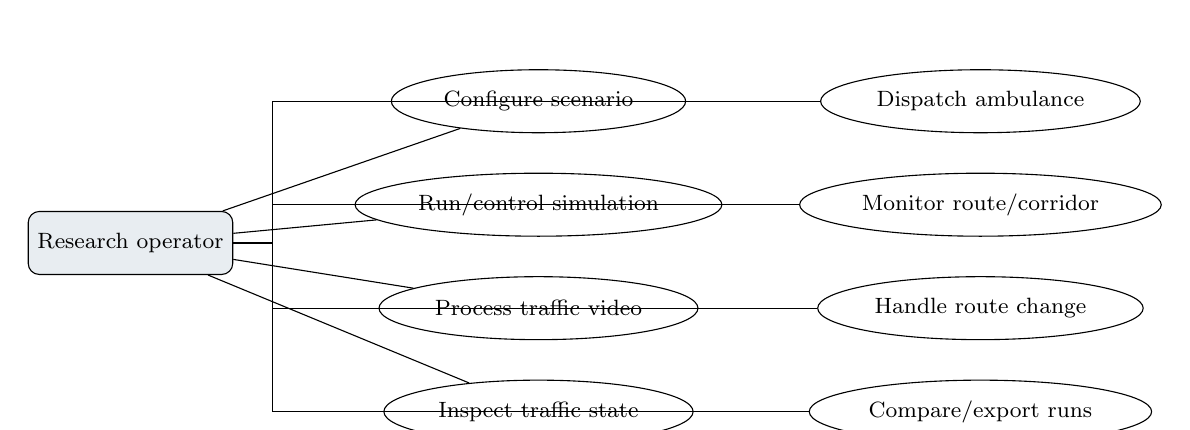
\begin{tikzpicture}[font=\footnotesize,uc/.style={draw,ellipse,minimum width=3.5cm,minimum height=0.8cm,align=center},actor/.style={draw,rounded corners,fill=manzilblue!10,minimum width=1.8cm,minimum height=0.8cm},node distance=5mm and 11mm]
\node[actor] (op) {Research operator};
\node[uc,right=20mm of op,yshift=18mm] (cfg) {Configure scenario};
\node[uc,below=of cfg] (run) {Run/control simulation};
\node[uc,below=of run] (video) {Process traffic video};
\node[uc,below=of video] (inspect) {Inspect traffic state};
\node[uc,right=17mm of cfg] (dispatch) {Dispatch ambulance};
\node[uc,below=of dispatch] (corr) {Monitor route/corridor};
\node[uc,below=of corr] (reroute) {Handle route change};
\node[uc,below=of reroute] (compare) {Compare/export runs};
\foreach \x in {cfg,run,video,inspect}{\draw (op)--(\x);}
\draw (op.east) -- ++(5mm,0) |- (dispatch.west);
\draw (op.east) -- ++(5mm,0) |- (corr.west);
\draw (op.east) -- ++(5mm,0) |- (reroute.west);
\draw (op.east) -- ++(5mm,0) |- (compare.west);
\end{tikzpicture}
\caption{Proposed operator use-case diagram}
\label{fig:use-case}
\end{figure}

\newcommand{\uctable}[7]{%
\begin{table}[H]\centering
\caption{#2}\label{#1}
\begin{tabularx}{\textwidth}{p{0.22\textwidth}Y}
\toprule
\textbf{Name / actor} & #2 / Research operator\\
\textbf{Preconditions} & #3\\
\textbf{Trigger} & #4\\
\textbf{Main success flow} & #5\\
\textbf{Alternative/failure flow} & #6\\
\textbf{Postconditions} & #7\\
\bottomrule
\end{tabularx}\end{table}}

\uctable{tab:uc1}{UC-01 Configure a scenario}{Network and controller descriptors are available.}{Operator requests a new experiment.}{Select network, demand, controller, seed, warm-up, duration, source mode, incident, and optional mission; validate; store a draft configuration.}{Reject incompatible controller/network, invalid duration, missing seed, or inaccessible input with field-specific messages.}{A valid, versioned configuration is ready; no run has started.}

\uctable{tab:uc2}{UC-02 Run and control a simulation}{UC-01 is valid; SUMO adapter is available.}{Operator selects Start.}{Create run record; launch SUMO; complete warm-up; step the simulation; collect state; request and apply lawful actions; publish snapshots; stop at terminal condition.}{If launch/TraCI fails, mark failed and retain logs. Pause/resume does not create competing clock owners. Invalid controller action invokes fallback.}{Run is completed, stopped, or failed with an explicit reason.}

\uctable{tab:uc3}{UC-03 Process traffic video}{Licensed video and model configuration are available.}{Operator selects a video job.}{Validate source; decode frames; detect vehicles; associate tracks; map valid tracks to regions; aggregate interval observations; store metrics and job status.}{Unreadable media, unsupported format, model failure, missing calibration, or low-confidence observation is reported; physical queue length is omitted when calibration is unavailable.}{Completed observations identify source, model, interval, units, and confidence.}

\uctable{tab:uc4}{UC-04 Inspect traffic state}{A run or perception job has emitted data.}{Operator opens overview or intersection detail.}{Display source mode, freshness, counts, queues/proxies, speeds, phases, controller, and warnings; allow time/intersection selection.}{Disconnected or stale streams remain visibly marked; last value is not presented as current.}{No system decision is changed; the inspected state is traceable to its source.}

\uctable{tab:uc5}{UC-05 Dispatch an ambulance}{A running emergency-enabled scenario exists.}{Operator submits origin and destination.}{Validate accessible edges; create mission; compute route/cost; assign simulated ambulance; publish route; request bounded corridor look-ahead.}{Invalid edge or no route returns a reason without partial priority. Duplicate active mission is rejected in the core single-ambulance mode.}{Mission is active with a valid current route, or rejected cleanly.}

\uctable{tab:uc6}{UC-06 Monitor route and corridor}{An emergency mission is active.}{Ambulance advances through the network.}{Update position and remaining path; request safe transition ahead; display corridor states; detect passage; release and recover each intersection.}{Missing vehicle, stale position, unsafe request, or corridor timeout triggers cancellation/fallback and a visible alert.}{Mission progress and all priority transitions are recorded.}

\uctable{tab:uc7}{UC-07 Handle blockage or changed route}{An active mission has a feasible current position.}{Closure or sustained cost change triggers evaluation.}{Recompute path from a valid remaining edge; compare benefits; if threshold is met, atomically revise route, cancel obsolete requests, and activate new look-ahead.}{If improvement is too small, retain route. If no route exists, cancel upcoming priority and mark mission blocked.}{Exactly one route version is current; every revision has cause and cost snapshot.}

\uctable{tab:uc8}{UC-08 Compare and export runs}{At least two completed or failed run records exist.}{Operator selects runs and metrics.}{Check comparability; align metric definitions; present distributions and configuration differences; export selected records.}{Warn or refuse direct comparison when network, demand, duration, warm-up, or metric version differs. Failed runs are not silently omitted.}{Comparison and export identify source run IDs and schema version.}

\section{Proposed Graphical User Interface}
\label{sec:gui}

The following figures are proposed wireframes, not screenshots of implemented software. Their purpose is to validate information hierarchy and required operator actions without fabricating progress.

\begin{figure}[H]
\centering
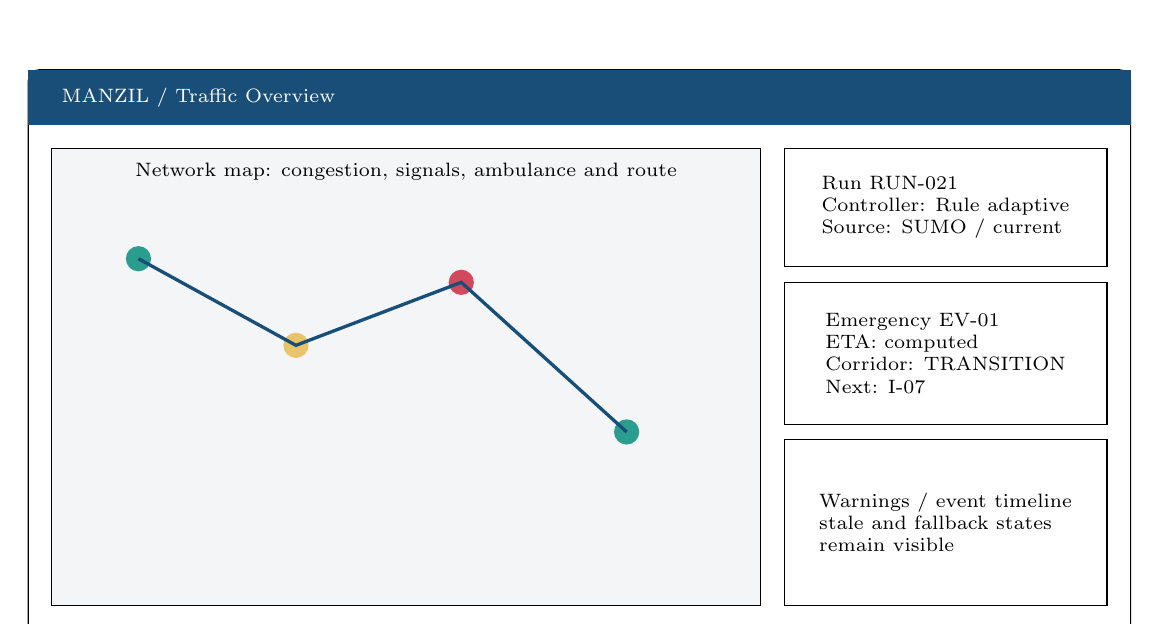
\begin{tikzpicture}[x=1cm,y=1cm,font=\scriptsize]
\draw[rounded corners] (0,0) rectangle (14,7.2);
\fill[manzilblue] (0,6.5) rectangle (14,7.2); \node[text=white,anchor=west] at (.3,6.85) {MANZIL / Traffic Overview};
\draw[fill=manzilgray] (.3,.4) rectangle (9.3,6.2); \node at (4.8,5.9) {Network map: congestion, signals, ambulance and route};
\foreach \x/\y/\c in {1.4/4.8/manzilgreen,3.4/3.7/manzilamber,5.5/4.5/manzilred,7.6/2.6/manzilgreen}{\fill[\c] (\x,\y) circle (.16);}
\draw[very thick,manzilblue] (1.4,4.8)--(3.4,3.7)--(5.5,4.5)--(7.6,2.6);
\draw (9.6,4.7) rectangle (13.7,6.2); \node[align=left] at (11.65,5.45) {Run RUN-021\\Controller: Rule adaptive\\Source: SUMO / current};
\draw (9.6,2.7) rectangle (13.7,4.5); \node[align=left] at (11.65,3.6) {Emergency EV-01\\ETA: computed\\Corridor: TRANSITION\\Next: I-07};
\draw (9.6,.4) rectangle (13.7,2.5); \node[align=left] at (11.65,1.45) {Warnings / event timeline\\stale and fallback states\\remain visible};
\end{tikzpicture}
\caption{Proposed traffic overview wireframe}
\label{fig:wire-overview}
\end{figure}

\begin{figure}[H]
\centering
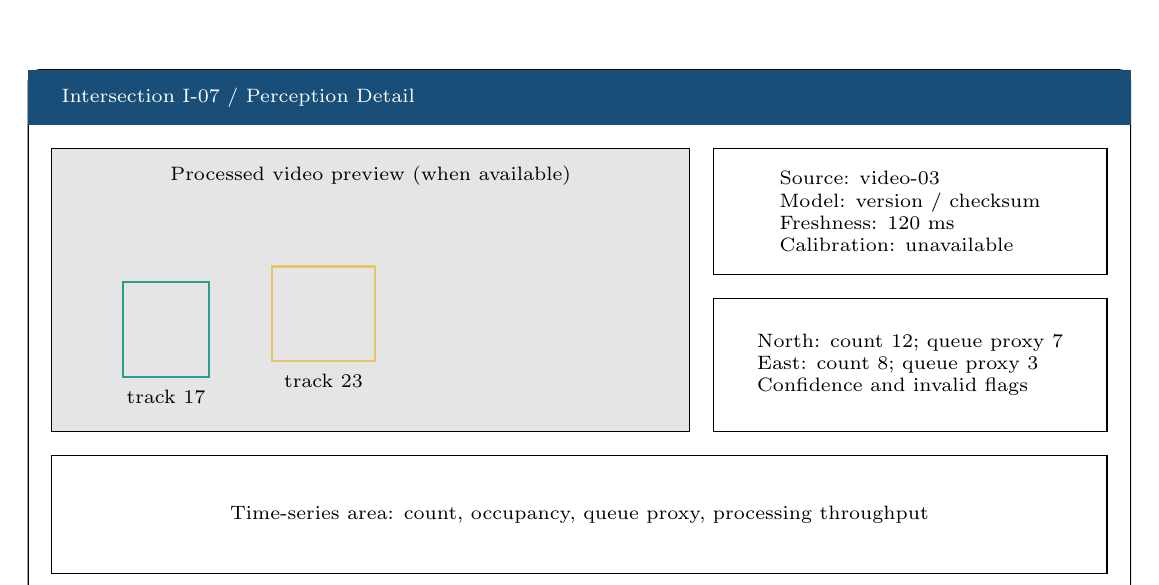
\begin{tikzpicture}[x=1cm,y=1cm,font=\scriptsize]
\draw[rounded corners] (0,0) rectangle (14,6.7);
\fill[manzilblue] (0,6) rectangle (14,6.7); \node[text=white,anchor=west] at (.3,6.35) {Intersection I-07 / Perception Detail};
\draw[fill=black!10] (.3,2.1) rectangle (8.4,5.7); \node at (4.35,5.35) {Processed video preview (when available)};
\draw[manzilgreen,thick] (1.2,2.8) rectangle (2.3,4.0); \node at (1.75,2.55) {track 17};
\draw[manzilamber,thick] (3.1,3.0) rectangle (4.4,4.2); \node at (3.75,2.75) {track 23};
\draw (8.7,4.1) rectangle (13.7,5.7); \node[align=left] at (11.2,4.9) {Source: video-03\\Model: version / checksum\\Freshness: 120 ms\\Calibration: unavailable};
\draw (8.7,2.1) rectangle (13.7,3.8); \node[align=left] at (11.2,2.95) {North: count 12; queue proxy 7\\East: count 8; queue proxy 3\\Confidence and invalid flags};
\draw (.3,.3) rectangle (13.7,1.8); \node at (7,1.05) {Time-series area: count, occupancy, queue proxy, processing throughput};
\end{tikzpicture}
\caption{Proposed perception and intersection-detail wireframe}
\label{fig:wire-perception}
\end{figure}

\begin{figure}[H]
\centering
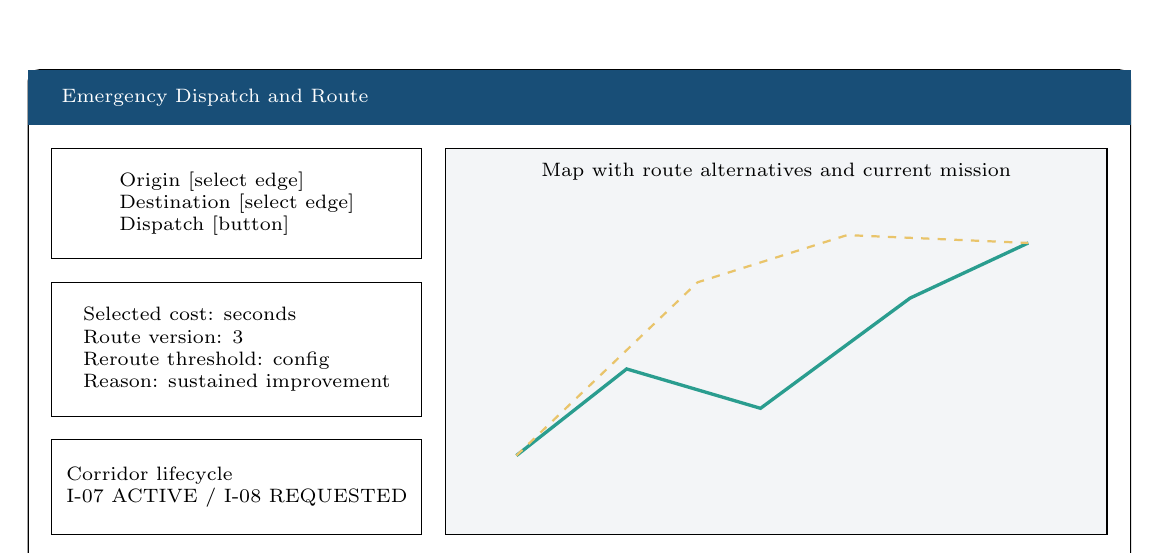
\begin{tikzpicture}[x=1cm,y=1cm,font=\scriptsize]
\draw[rounded corners] (0,0) rectangle (14,6.3);
\fill[manzilblue] (0,5.6) rectangle (14,6.3); \node[text=white,anchor=west] at (.3,5.95) {Emergency Dispatch and Route};
\draw (.3,3.9) rectangle (5.0,5.3); \node[align=left] at (2.65,4.6) {Origin [select edge]\\Destination [select edge]\\Dispatch [button]};
\draw[fill=manzilgray] (5.3,.4) rectangle (13.7,5.3); \node at (9.5,5.0) {Map with route alternatives and current mission};
\draw[very thick,manzilgreen] (6.2,1.4)--(7.6,2.5)--(9.3,2.0)--(11.2,3.4)--(12.7,4.1);
\draw[thick,dashed,manzilamber] (6.2,1.4)--(8.5,3.6)--(10.4,4.2)--(12.7,4.1);
\draw (.3,1.9) rectangle (5,3.6); \node[align=left] at (2.65,2.75) {Selected cost: seconds\\Route version: 3\\Reroute threshold: config\\Reason: sustained improvement};
\draw (.3,.4) rectangle (5,1.6); \node[align=left] at (2.65,1.0) {Corridor lifecycle\\I-07 ACTIVE / I-08 REQUESTED};
\end{tikzpicture}
\caption{Proposed emergency dispatch and route wireframe}
\label{fig:wire-dispatch}
\end{figure}

\begin{figure}[H]
\centering
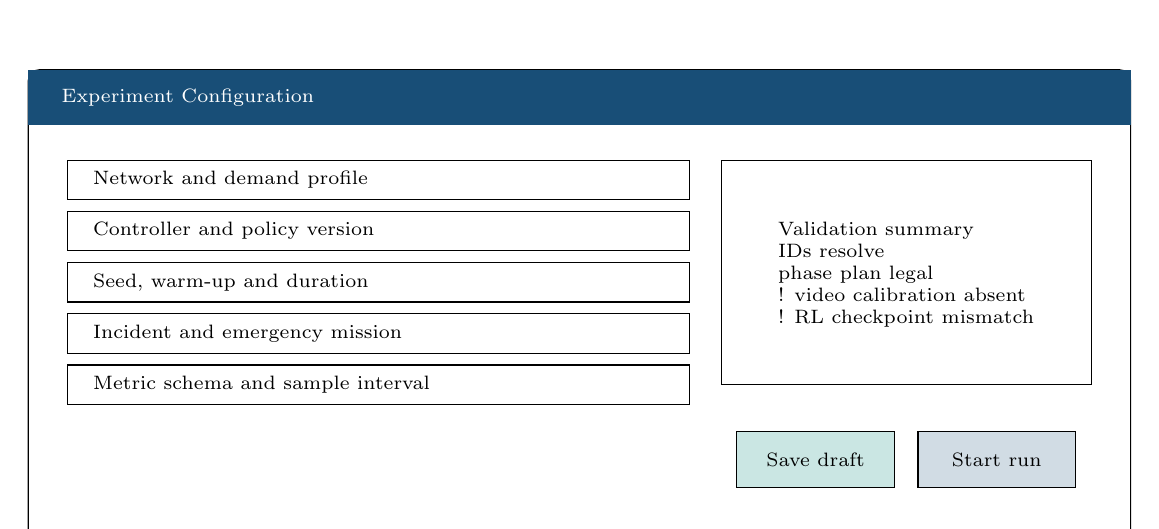
\begin{tikzpicture}[x=1cm,y=1cm,font=\scriptsize]
\draw[rounded corners] (0,0) rectangle (14,6);
\fill[manzilblue] (0,5.3) rectangle (14,6); \node[text=white,anchor=west] at (.3,5.65) {Experiment Configuration};
\draw (.5,4.35) rectangle (8.4,4.85); \node[anchor=west] at (.7,4.6) {Network and demand profile};
\draw (.5,3.70) rectangle (8.4,4.20); \node[anchor=west] at (.7,3.95) {Controller and policy version};
\draw (.5,3.05) rectangle (8.4,3.55); \node[anchor=west] at (.7,3.30) {Seed, warm-up and duration};
\draw (.5,2.40) rectangle (8.4,2.90); \node[anchor=west] at (.7,2.65) {Incident and emergency mission};
\draw (.5,1.75) rectangle (8.4,2.25); \node[anchor=west] at (.7,2.00) {Metric schema and sample interval};
\draw (8.8,2.0) rectangle (13.5,4.85); \node[align=left] at (11.15,3.4) {Validation summary\\\checkmark IDs resolve\\\checkmark phase plan legal\\! video calibration absent\\! RL checkpoint mismatch};
\draw[fill=manzilgreen!25] (9.0,.7) rectangle (11.0,1.4); \node at (10,1.05) {Save draft};
\draw[fill=manzilblue!20] (11.3,.7) rectangle (13.3,1.4); \node at (12.3,1.05) {Start run};
\end{tikzpicture}
\caption{Proposed experiment-configuration wireframe}
\label{fig:wire-config}
\end{figure}

\begin{figure}[H]
\centering
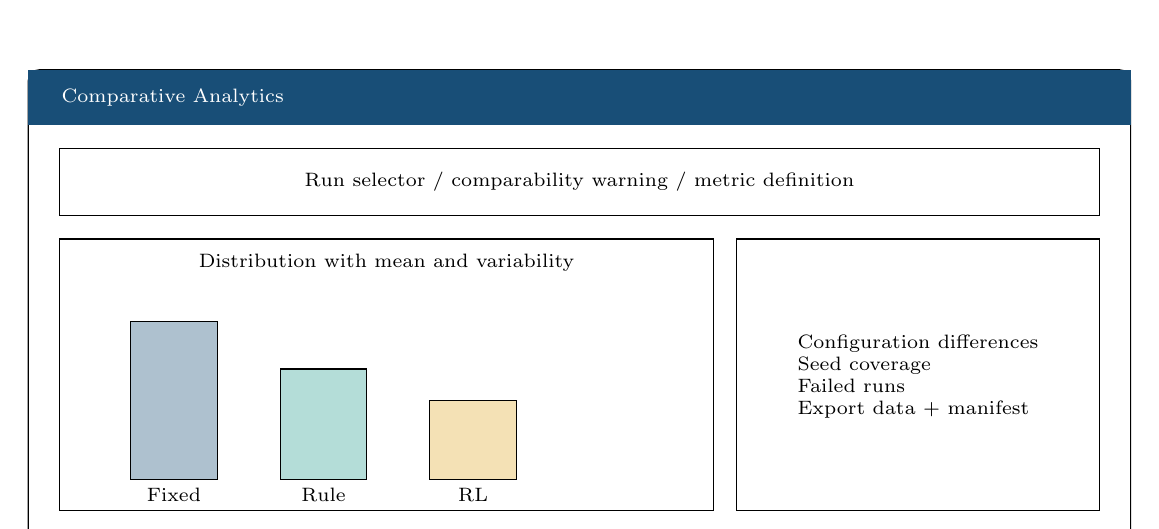
\begin{tikzpicture}[x=1cm,y=1cm,font=\scriptsize]
\draw[rounded corners] (0,0) rectangle (14,6);
\fill[manzilblue] (0,5.3) rectangle (14,6); \node[text=white,anchor=west] at (.3,5.65) {Comparative Analytics};
\draw (.4,4.15) rectangle (13.6,5.0); \node at (7,4.58) {Run selector / comparability warning / metric definition};
\draw (.4,.4) rectangle (8.7,3.85); \node at (4.55,3.55) {Distribution with mean and variability};
\draw[fill=manzilblue!35] (1.3,.8) rectangle (2.4,2.8); \draw[fill=manzilgreen!35] (3.2,.8) rectangle (4.3,2.2); \draw[fill=manzilamber!50] (5.1,.8) rectangle (6.2,1.8);
\node at (1.85,.6) {Fixed}; \node at (3.75,.6) {Rule}; \node at (5.65,.6) {RL};
\draw (9.0,.4) rectangle (13.6,3.85); \node[align=left] at (11.3,2.1) {Configuration differences\\Seed coverage\\Failed runs\\Export data + manifest};
\end{tikzpicture}
\caption{Proposed comparative-analytics wireframe; bars are schematic and not results}
\label{fig:wire-analytics}
\end{figure}

\section{Data Design}
\label{sec:data-design}

Persistent data is reserved for configuration, observations, decisions, missions, and outcomes that require audit or comparison. The live road graph, current TraCI subscription, and frame buffers are in-memory runtime state. Raw video remains an external file with a content identifier rather than a database blob.

\begin{figure}[H]
\centering
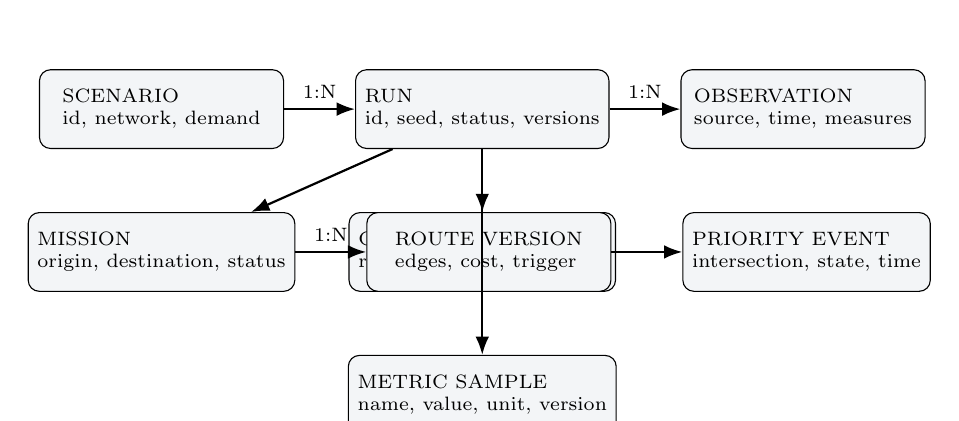
\begin{tikzpicture}[font=\scriptsize,node distance=8mm and 9mm,ent/.style={draw,rounded corners,fill=manzilgray,minimum width=3.1cm,minimum height=1.0cm,align=left},rel/.style={-{Latex},thick}]
\node[ent] (scenario) {SCENARIO\\id, network, demand};
\node[ent,right=of scenario] (run) {RUN\\id, seed, status, versions};
\node[ent,right=of run] (obs) {OBSERVATION\\source, time, measures};
\node[ent,below=of run] (decision) {CONTROL DECISION\\requested/applied, reason};
\node[ent,below=of scenario] (mission) {MISSION\\origin, destination, status};
\node[ent,right=of mission] (route) {ROUTE VERSION\\edges, cost, trigger};
\node[ent,right=of route] (priority) {PRIORITY EVENT\\intersection, state, time};
\node[ent,below=of decision] (metric) {METRIC SAMPLE\\name, value, unit, version};
\draw[rel] (scenario)--node[above]{1:N}(run);
\draw[rel] (run)--node[above]{1:N}(obs);
\draw[rel] (run)--(decision); \draw[rel] (run)--(metric);
\draw[rel] (run)--(mission); \draw[rel] (mission)--node[above]{1:N}(route);
\draw[rel] (route)--(priority);
\end{tikzpicture}
\caption{Proposed experiment-record entity relationship model}
\label{fig:er}
\end{figure}

\begin{longtable}{p{0.19\textwidth}p{0.22\textwidth}p{0.48\textwidth}}
\caption{Data dictionary}\label{tab:data-dictionary}\\
\toprule
\textbf{Entity} & \textbf{Key fields} & \textbf{Integrity rule}\\
\midrule\endfirsthead
\toprule
\textbf{Entity} & \textbf{Key fields} & \textbf{Integrity rule}\\
\midrule\endhead
Scenario & scenario\_id, network\_version, demand\_version & References immutable network and demand manifests.\\
Run & run\_id, scenario\_id, seed, controller\_version, status & Configuration becomes immutable after start; terminal reason required.\\
Observation & run\_id/job\_id, source\_mode, entity\_id, observed\_at, valid\_until, values, units & Source and units are mandatory; validity interval cannot be inferred.\\
ControlDecision & run\_id, intersection\_id, requested\_phase, applied\_phase, effective\_step, reason & Requested and applied actions are separate fields.\\
Mission & mission\_id, run\_id, vehicle\_id, origin, destination, status & Only one active core mission per run.\\
RouteVersion & mission\_id, version, edge\_list, cost\_seconds, trigger, created\_at & Version increases monotonically; path begins at valid current position.\\
PriorityEvent & mission\_id, route\_version, intersection\_id, state, requested/applied time & References the route version that justified priority.\\
MetricSample & run\_id, metric\_name, metric\_version, value, unit, interval & Comparisons require matching metric name, version, and unit.\\
Artifact & run/job\_id, type, URI, checksum, license/provenance & Content is addressable and provenance is retained.\\
\bottomrule
\end{longtable}

\section{Risk Analysis}

\small
\begin{longtable}{p{0.20\textwidth}p{0.10\textwidth}p{0.10\textwidth}p{0.28\textwidth}p{0.13\textwidth}}
\caption{Risk register}\label{tab:risks}\\
\toprule
\textbf{Risk} & \textbf{Likelihood} & \textbf{Impact} & \textbf{Mitigation} & \textbf{Fallback}\\
\midrule\endfirsthead
Map import lacks valid signals/turns & Medium & High & Inspect and clean a small extract early; validate routes and phases & Use a documented synthetic grid\\
Local video lacks labels or permission & Medium & High & Use licensed public sequences and record provenance & Evaluate public data only; state domain gap\\
Occlusion causes unstable counts & High & Medium & Region rules, temporal aggregation, tracker comparison & Limit claims to labelled conditions\\
RL fails to converge or generalize & Medium & High & Stable baselines, bounded action space, tune only on training scenarios & Report baseline comparison; treat RL as negative/partial finding\\
Reward improves one metric unfairly & Medium & High & Multi-metric evaluation and starvation constraints & Reject policy violating safety or fairness checks\\
Rerouting oscillates & Medium & Medium & Benefit threshold, persistence, cooldown, closure exception & Freeze current feasible route\\
Preemption leaves unsafe phase & Low & Very high & Central state machine and invariant tests & Cancel request and use safe baseline transition\\
Service timing drifts from simulation & Medium & High & One step owner, simulation timestamps, bounded queues & Run synchronously without live perception\\
Insufficient compute & Medium & Medium & Profile early; smaller network/model and offline training & Demonstrate recorded inference and compact scenarios\\
Results are not reproducible & Medium & High & Immutable manifests, seeds, versioned metrics and exports & Exclude untraceable runs\\
\bottomrule
\end{longtable}
\normalsize

\section{Requirements Traceability}

\begin{longtable}{p{0.15\textwidth}p{0.20\textwidth}p{0.27\textwidth}p{0.20\textwidth}}
\caption{Requirements traceability matrix}\label{tab:traceability}\\
\toprule
\textbf{Requirements} & \textbf{Use cases} & \textbf{Design modules} & \textbf{Planned verification}\\
\midrule\endfirsthead
\toprule
\textbf{Requirements} & \textbf{Use cases} & \textbf{Design modules} & \textbf{Planned verification}\\
\midrule\endhead
FR-01, 17--19; NFR-01,10 & UC-01, UC-08 & Experiment service, store & Schema, validation, replay and comparison tests\\
FR-02,03,07; NFR-02,06 & UC-02 & Simulation adapter, control orchestrator & Single-owner and phase-invariant tests\\
FR-04,05; NFR-04,11 & UC-03, UC-04 & Perception worker, state aggregator & Annotated sequence evaluation and stale-data tests\\
FR-06,08,20 & UC-02 & Controller interface, safety filter & Fixed scenarios, illegal-action and fallback tests\\
FR-09--11,14 & UC-05, UC-07 & Graph/routing service & Disconnected graph, closure, hysteresis and path-validity tests\\
FR-12,13 & UC-06, UC-07 & Corridor coordinator & Lifecycle, timeout, cancellation and recovery tests\\
FR-15,16 & UC-04, UC-06 & API gateway, dashboard & UI state and warning acceptance checks\\
NFR-03,05,07--09,12 & All & Cross-cutting contracts and deployment & Log audit, profiling, usability walkthrough, failure injection\\
\bottomrule
\end{longtable}

\section{Conclusion}

The specification centers on traceability and failure visibility. It requires one simulation-clock owner, legal signal transitions, stable route revision, explicit source freshness, reproducible run records, and comparisons that cannot hide incompatible configurations. These requirements become procedural and architectural choices in the next two chapters.

\chapter{Proposed Approach and Methodology}
\label{ch:method}

This chapter defines how Manzil will be constructed and evaluated. The methodology is designed to answer the research questions with controlled comparisons, not to optimize a demonstration for a favorable single run. Figure \ref{fig:method-workflow} summarizes the sequence from preparation to evidence.

\section{Overall Research Workflow}

\begin{figure}[H]
\centering
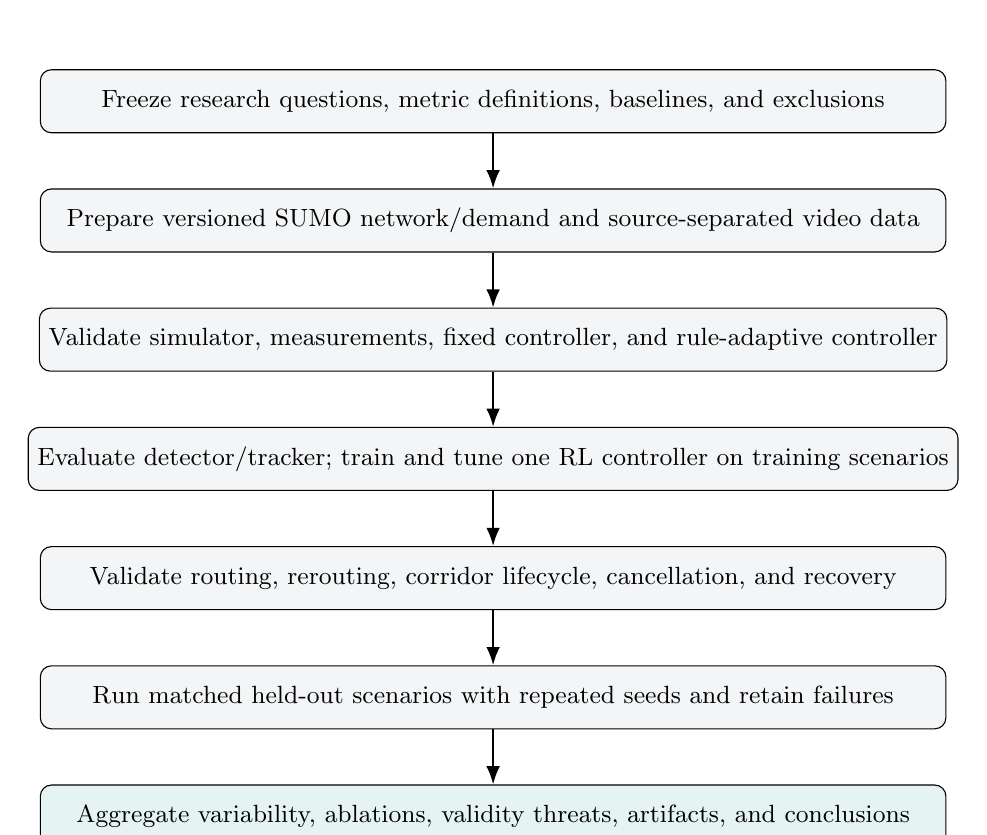
\begin{tikzpicture}[font=\small,node distance=7mm,box/.style={draw,rounded corners,fill=manzilgray,minimum width=11.5cm,minimum height=.8cm,align=center},arr/.style={-{Latex},thick}]
\node[box] (q) {Freeze research questions, metric definitions, baselines, and exclusions};
\node[box,below=of q] (prep) {Prepare versioned SUMO network/demand and source-separated video data};
\node[box,below=of prep] (base) {Validate simulator, measurements, fixed controller, and rule-adaptive controller};
\node[box,below=of base] (models) {Evaluate detector/tracker; train and tune one RL controller on training scenarios};
\node[box,below=of models] (em) {Validate routing, rerouting, corridor lifecycle, cancellation, and recovery};
\node[box,below=of em] (eval) {Run matched held-out scenarios with repeated seeds and retain failures};
\node[box,below=of eval,fill=manzilgreen!12] (report) {Aggregate variability, ablations, validity threats, artifacts, and conclusions};
\draw[arr] (q)--(prep);\draw[arr] (prep)--(base);\draw[arr] (base)--(models);\draw[arr] (models)--(em);\draw[arr] (em)--(eval);\draw[arr] (eval)--(report);
\end{tikzpicture}
\caption{Proposed research and evaluation workflow}
\label{fig:method-workflow}
\end{figure}

Two input modes are retained. In \emph{video mode}, annotations supply the reference for perception metrics and no claim is made that video determines the full selected road network. In \emph{simulation mode}, SUMO supplies exact lane, vehicle, signal, and route state for control experiments. A future noise study may inject measured perception error into the simulation-state contract, but it will be included only if the baseline experiments are complete and the protocol is fixed in advance.

\section{Network and Scenario Preparation}

\subsection{Network Provenance and Validation}

A selected, manageable Lahore road area will be exported from OpenStreetMap under its applicable attribution and license conditions \cite{osmlicense}. The exact bounding box, extraction date, source file checksum, and conversion command will be stored. SUMO's import toolchain will convert the graph, after which NetEdit inspection will verify lane counts, legal turns, junction types, traffic-light programs, pedestrian-only edges, disconnected components, and ambulance-accessible routes.

The initial size target from project context is approximately 10--20 signalized intersections, but this remains a planning range rather than a confirmed network fact. A smaller validated extract is preferable to a larger inaccurate one. If import quality prevents stable experiments within the schedule, a synthetic multi-intersection grid with documented geometry and demand becomes the fallback; results will be identified as synthetic.

\subsection{Demand and Incidents}

Demand files will define light, medium, and heavy conditions plus an uneven approach case. Vehicle insertion will use explicit random seeds. The warm-up period allows the network to reach a representative occupancy before measurements. Incident scenarios will close an edge, reduce lane capacity, or insert a controlled obstruction at a declared simulation time. A failed insertion due to a full lane will be recorded rather than retried until a favorable run occurs.

The same demand realization will be replayed across controllers where SUMO semantics permit. If a controller changes route choices or insertion feasibility, the manifest will distinguish the original demand request from actual departures. Scenario families will be separated into development, tuning, and held-out evaluation sets.

\section{Video Perception Pipeline}

\begin{figure}[H]
\centering
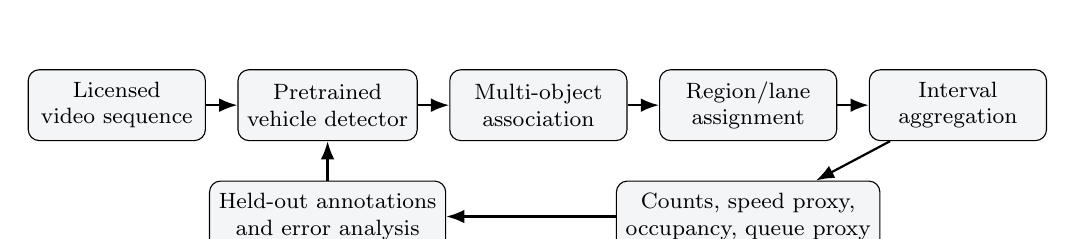
\begin{tikzpicture}[font=\footnotesize,node distance=5mm and 4mm,box/.style={draw,rounded corners,fill=manzilgray,minimum width=2.25cm,minimum height=.9cm,align=center},arr/.style={-{Latex},thick}]
\node[box] (v) {Licensed\\video sequence};
\node[box,right=of v] (d) {Pretrained\\vehicle detector};
\node[box,right=of d] (t) {Multi-object\\association};
\node[box,right=of t] (g) {Region/lane\\assignment};
\node[box,right=of g] (a) {Interval\\aggregation};
\node[box,below=of g] (m) {Counts, speed proxy,\\occupancy, queue proxy};
\node[box,below=of d] (e) {Held-out annotations\\and error analysis};
\draw[arr] (v)--(d);\draw[arr] (d)--(t);\draw[arr] (t)--(g);\draw[arr] (g)--(a);\draw[arr] (a)--(m);\draw[arr] (e)--(d);\draw[arr] (m)--(e);
\end{tikzpicture}
\caption{Proposed traffic-video perception pipeline}
\label{fig:perception}
\end{figure}

As Figure \ref{fig:perception} shows, the detector produces class, confidence, and image coordinates; the tracker assigns a temporary identity; and a bottom-center or calibrated road-contact point assigns each track to a polygonal region. Counts use a directed line-crossing or region-entry rule and track history to avoid frame-wise duplication. A speed in physical units requires camera calibration or known scale. Without calibration, the system reports pixel displacement or a categorical slow/stationary state, not kilometres per hour.

For a lane region $l$ over interval $k$, a simple occupancy proxy is
\begin{equation}
O_{l,k}=\frac{1}{T_k}\sum_{t\in k}\frac{\sum_{i\in V_{l,t}} A(B_{i,t}\cap R_l)}{A(R_l)},
\end{equation}
where $B_{i,t}$ is a tracked box, $R_l$ is the image region, and $T_k$ is the number of sampled frames. This is image occupancy, not road density. A queue proxy counts stable tracks inside a defined upstream region whose image-motion or calibrated speed is below a threshold for a minimum persistence time.

The detector will be initialized from a documented pretrained checkpoint, consistent with the practical motivation of YOLO-family detection \cite{redmon2016yolo}. ByteTrack is the leading proposed tracker because its low-score association may reduce occlusion fragmentation \cite{zhang2022bytetrack}; DeepSORT remains a comparison if appearance association materially improves the selected scenes \cite{wojke2017deepsort}. The final choice will be based on the held-out count and tracking requirements, not benchmark reputation.

\section{Normal Traffic Controllers}

\subsection{Fixed-Time Controller}

The fixed controller will use a declared cycle and phase sequence appropriate to the selected junction. Green, yellow, and all-red durations and offsets will be versioned. It will not be intentionally starved or given unrealistic timing to make adaptive methods appear superior. A basic saturation check will ensure that at least the light scenario is serviceable.

\subsection{Rule-Based Adaptive Controller}

The initial transparent controller evaluates only legal candidate phases. A pressure-inspired score for phase $p$ is
\begin{equation}
S_p(t)=\sum_{(l,m)\in p}\left(q_l(t)-\alpha q_m(t)\right)+\beta w_l(t),
\label{eq:rule-score}
\end{equation}
where $q_l$ and $q_m$ are upstream and downstream queues for a served movement, $w_l$ is the maximum accumulated wait among its approaches, and $\alpha,\beta$ are documented configuration values. This follows the motivation of max-pressure control \cite{varaiya2013maxpressure} while retaining a direct anti-starvation term.

At each decision instant, the current green is held until minimum green. A phase may be extended if it remains best and maximum green is not reached. A phase whose maximum red exceeds a limit is promoted. Switching inserts the same clearance sequence used by all controllers. No controller can directly bypass the safety filter.

\subsection{Proposed RL Formulation}

One RL formulation will be selected after the rule baseline is stable. A feasible initial choice is a discrete-action value-based policy for a small, fixed phase set; pressure-informed reward design is supported by PressLight \cite{wei2019presslight}. If the network needs coordinated agents and the training budget permits, centralized observations with per-intersection actions are preferred over loosely defined independent learners.

The proposed state for each decision interval includes normalized incoming and outgoing queues, approach waiting time, occupancy, current phase, elapsed phase time, and an emergency-mode flag. An action requests a legal phase or a bounded extension. The safety layer remains authoritative. A candidate reward is
\begin{equation}
r_t=-\lambda_p P_t-\lambda_w W_t-\lambda_s X_t-\lambda_c C_t,
\label{eq:reward}
\end{equation}
where $P_t$ is network pressure, $W_t$ normalized waiting, $X_t$ a starvation violation, and $C_t$ an unnecessary-switch penalty. Coefficients and normalization will be fixed on training/tuning scenarios. Emergency performance is evaluated in a separate supervisory experiment so that the first normal-controller comparison is not confounded by rare mission rewards.

Training will record episode seed, demand profile, exploration schedule, optimizer settings, network checksum, reward components, and checkpoints. Evaluation uses deterministic policy settings where applicable and held-out demands. Training return alone is not an evaluation result.

\section{Dynamic Graph Routing}

The routing graph represents legal vehicle movements. Nodes may be junctions or lane/edge transition points; edges store length, allowed class, free-flow time, current travel-time estimate, queue discharge estimate, residual signal delay, closure state, and observation time. The exact representation will match SUMO route validity rather than an abstract map that permits illegal turns.

The primary edge cost is expressed in seconds:
\begin{equation}
c_e(t)=\hat{T}^{\mathrm{link}}_e(t)+\hat{D}^{\mathrm{signal}}_e(t)+\hat{D}^{\mathrm{queue}}_e(t)+M_e(t),
\label{eq:edgecost}
\end{equation}
where $M_e(t)=0$ for an open edge and infinity for a hard closure. Queue delay is included only if it is not already represented in the link travel-time estimate. Every cost snapshot records source and freshness.

Dijkstra's algorithm provides the reference minimum-cost path under nonnegative weights \cite{dijkstra1959}. A* is permitted with $h(n)$ equal to a lower bound based on straight-line distance divided by the maximum allowed free-flow speed; this remains no greater than true time when added delays are nonnegative \cite{hart1968astar}. If that condition cannot be guaranteed, Dijkstra is retained.

\begin{algorithm}[H]
\caption{Congestion-aware route selection and stable rerouting}
\label{alg:routing}
\KwData{Current ambulance edge $s$, destination $g$, current route $R$, cost snapshot $C_t$}
\KwResult{Retained or revised valid remaining route}
Reject stale or negative costs; apply closures to $C_t$\;
$R'\leftarrow \mathrm{ShortestPath}(s,g,C_t)$\;
\If{$R'$ does not exist}{return NO\_ROUTE and cancel future corridor requests\;}
Compute remaining costs $J(R)$ and $J(R')$ under the same snapshot\;
\eIf{current route is infeasible}{accept $R'$ immediately\;}
{accept $R'$ only if $J(R)-J(R')>\delta$ for persistence window $\tau$ and cooldown has elapsed\;}
Validate route continuity from the current position\;
Atomically increment route version, cancel obsolete priority, and publish the revision\;
\end{algorithm}

The improvement threshold $\delta$, persistence $\tau$, and cooldown are configuration parameters to be tuned before held-out tests. This prevents small state fluctuations from producing route oscillation.

\section{Moving Green Corridor}

The corridor operates on a bounded number of route intersections ahead of the ambulance. Activation may use estimated time to arrival and queue clearance rather than a fixed distance alone. Each intersection receives a request containing mission ID, route version, approach movement, predicted arrival, expiry, and priority level.

Before serving the ambulance movement, the coordinator completes minimum green and applies the configured yellow and all-red clearance for conflicting movements. It does not set every route signal green at once. Passage is confirmed from the simulated vehicle position and lane transition, with a timeout as failure detection. After passage, the intersection enters recovery and either completes a bounded compensation plan or returns at a safe cycle boundary. A revised route cancels obsolete requests. These mechanisms follow the transition and recovery emphasis in emergency-preemption research \cite{qin2012preemption}.

\begin{algorithm}[H]
\caption{Corridor lifecycle at one intersection}
\label{alg:corridor}
\KwData{Priority request, ambulance state, signal state, safety configuration}
\If{request is stale, route version is obsolete, or movement is invalid}{reject and log reason\;}
Queue the request and estimate activation time\;
At activation, finish minimum green and apply legal clearance\;
Serve the ambulance movement within maximum priority duration\;
\If{passage is confirmed}{release and enter recovery\;}
\ElseIf{mission is cancelled, route changes, or timeout occurs}{cancel safely and enter recovery/fallback\;}
Restore normal controller ownership at a valid phase boundary and record recovery time\;
\end{algorithm}

The core scope contains one active ambulance, which avoids inventing an untested arbitration policy. Multiple emergency vehicles remain future work. Normal-traffic harm is bounded using a maximum priority duration, downstream occupancy check, and maximum-red monitoring. Exact limits are simulation parameters to be justified through sensitivity analysis, not field safety values.

\section{Integrated Control Loop}

\begin{algorithm}[H]
\caption{Single-owner simulation and decision loop}
\label{alg:loop}
\KwData{Validated run configuration and initialized services}
\While{run is active and before terminal simulation time}{
Advance SUMO by exactly one configured step\;
Read subscribed vehicle, lane, signal, and mission state\;
Construct a timestamped traffic-state snapshot\;
Update route costs and evaluate rerouting at its configured interval\;
Update corridor requests and lifecycle states\;
\eIf{corridor owns an intersection}{request its safe priority action\;}{request action from the selected normal controller\;}
Validate every requested action through the phase safety filter\;
Apply accepted actions through the TraCI adapter only\;
Record applied actions, events, and metric samples\;
Publish a non-authoritative dashboard snapshot\;
}
Finalize run status, artifacts, and checksums\;
\end{algorithm}

Algorithm \ref{alg:loop} makes event order explicit. Dashboard refresh and perception jobs cannot step the simulation. A snapshot used at time $t$ carries its effective step so that late data is either mapped deliberately or rejected.

\section{Experimental Protocol}

\subsection{Comparison Matrix}

\begin{table}[H]
\centering
\caption{Planned experiments and primary evidence}
\label{tab:experiments}
\begin{tabularx}{\textwidth}{p{0.20\textwidth}p{0.34\textwidth}Y}
\toprule
\textbf{Question} & \textbf{Controlled comparison} & \textbf{Primary measures}\\
\midrule
RQ1 perception & Detector/tracker output vs. held-out sequence annotations & Precision/recall or mAP where suitable; count MAE; identity metric only when required; queue-proxy error; throughput\\
RQ2 normal control & Fixed vs. rule-adaptive vs. selected RL under matched scenarios/seeds & Mean travel and waiting time, queue mean/max, throughput, phase changes, max-red/fairness violations\\
RQ3 routing & Static/reference route vs. dynamic route, holding signal policy fixed & Ambulance travel time, delay, stops, route revisions, computation time\\
RQ4 corridor & Same routing without vs. with corridor & Ambulance time/stops; ordinary traffic delay/queues; recovery time; safety invariant violations\\
RQ5 robustness & Demand, incident, seed, and optional observation-noise strata & Effect distributions and sensitivity; failed and no-route runs retained\\
\bottomrule
\end{tabularx}
\end{table}

\subsection{Scenario Assignment and Repetition}

The evaluation manifest will define demand levels, origin/destination pairs, incident timing, warm-up, measurement horizon, and repeated seeds before final runs. Every controller receives the same set. The number of repetitions will be chosen using pilot variance and available computation, then reported rather than retroactively reduced to favorable cases. Averages will be accompanied by standard deviation or confidence intervals, and paired differences will be used when runs share a demand seed.

RL training and hyperparameter selection use only training/tuning scenarios. Held-out demand combinations and at least one unseen seed set are reserved for final evaluation. Perception data is split by source or continuous sequence to reduce temporal leakage. The report will include failures, timeouts, infeasible routes, and safety-filter interventions.

\subsection{Metric Definitions}

For $N$ completed vehicles with travel times $T_i$, mean travel time is $\bar{T}=N^{-1}\sum_iT_i$. Queue length is sampled at fixed simulation intervals and reported as time mean and maximum by approach. Throughput is the number of vehicles crossing a declared network boundary during the measurement interval. Fairness includes maximum red time and approach-level delay distribution; an aggregate mean alone can conceal starvation.

Ambulance delay is actual travel time minus free-flow route time under the same network definition. Ordinary-traffic impact is evaluated on non-emergency vehicles and includes delay during the mission plus a recovery interval. Route computation time is measured separately from simulated travel time. For perception counts $y_k$ and estimates $\hat{y}_k$, mean absolute error is
\begin{equation}
\mathrm{MAE}=\frac{1}{K}\sum_{k=1}^{K}|y_k-\hat{y}_k|.
\end{equation}

\subsection{Reproducibility Package}

Each run will retain the source revision, dependency manifest, SUMO version, network and route checksums, controller/model version, full configuration, seed, logs, metric schema, and terminal reason. Large external video and pretrained weights may be referenced by license-aware URI and checksum. A script should recreate a run from its manifest; any manual NetEdit change must be committed as a network artifact.

\section{Threats to Validity}

\textbf{Construct validity} is threatened if queue proxies, waiting-time definitions, or reward components do not represent the intended concept. Definitions and units will be versioned, and perception proxies will not be renamed as physical quantities without calibration.

\textbf{Internal validity} is threatened by unmatched demand, different warm-up, hidden seed changes, or controller-specific failures. Paired manifests, one measurement implementation, and retention of failed runs mitigate these risks.

\textbf{External validity} is limited by synthetic demand, map inaccuracies, simulator car-following assumptions, and video domain shift. Findings will be bounded to the tested network, demand families, and video sources. No clinical response-time or public-road safety conclusion will be drawn.

\textbf{Conclusion validity} is threatened by few repetitions, tuning on the test set, and reporting only means. Pilot variance, held-out scenarios, paired comparisons, variability, and sensitivity analysis will be used. Statistical tests, if used, will name assumptions and effect sizes; significance alone will not establish practical value.

\section{Conclusion}

The methodology specifies a feasible progression from validated baselines to integrated emergency control. It uses time-consistent route costs, hysteresis, explicit corridor transitions, held-out evaluation, and reproducibility artifacts. Most importantly, it defines how negative or mixed results remain valid findings rather than prompting undocumented changes to the experiment.

\chapter{High-Level and Low-Level Design}
\label{ch:design}

This chapter maps the requirements and methodology to a service-oriented prototype design. The decomposition protects simulation determinism: one adapter owns the simulation clock and all signal actuation, while the API, dashboard, perception, controllers, and experiment store exchange typed messages without competing for control.

\section{System Overview and Design Goals}

The system must support repeatable research runs, interactive demonstrations, and post-run analysis. Its principal design goals are: deterministic ownership of state changes; replaceable controller and perception implementations; explicit time, units, and validity; safe corridor transitions; immutable experimental configuration; and visible failure. Performance is important only after these properties are preserved.

The design assumes a single machine or small development deployment for Deliverable 2/FYP-I. Separating components logically does not require premature distribution. In-process modules may be used initially behind the same interfaces, then isolated as workers if profiling justifies it.

\section{High-Level Architecture}
\label{sec:architecture}

\begin{figure}[H]
\centering
\resizebox{\textwidth}{!}{%
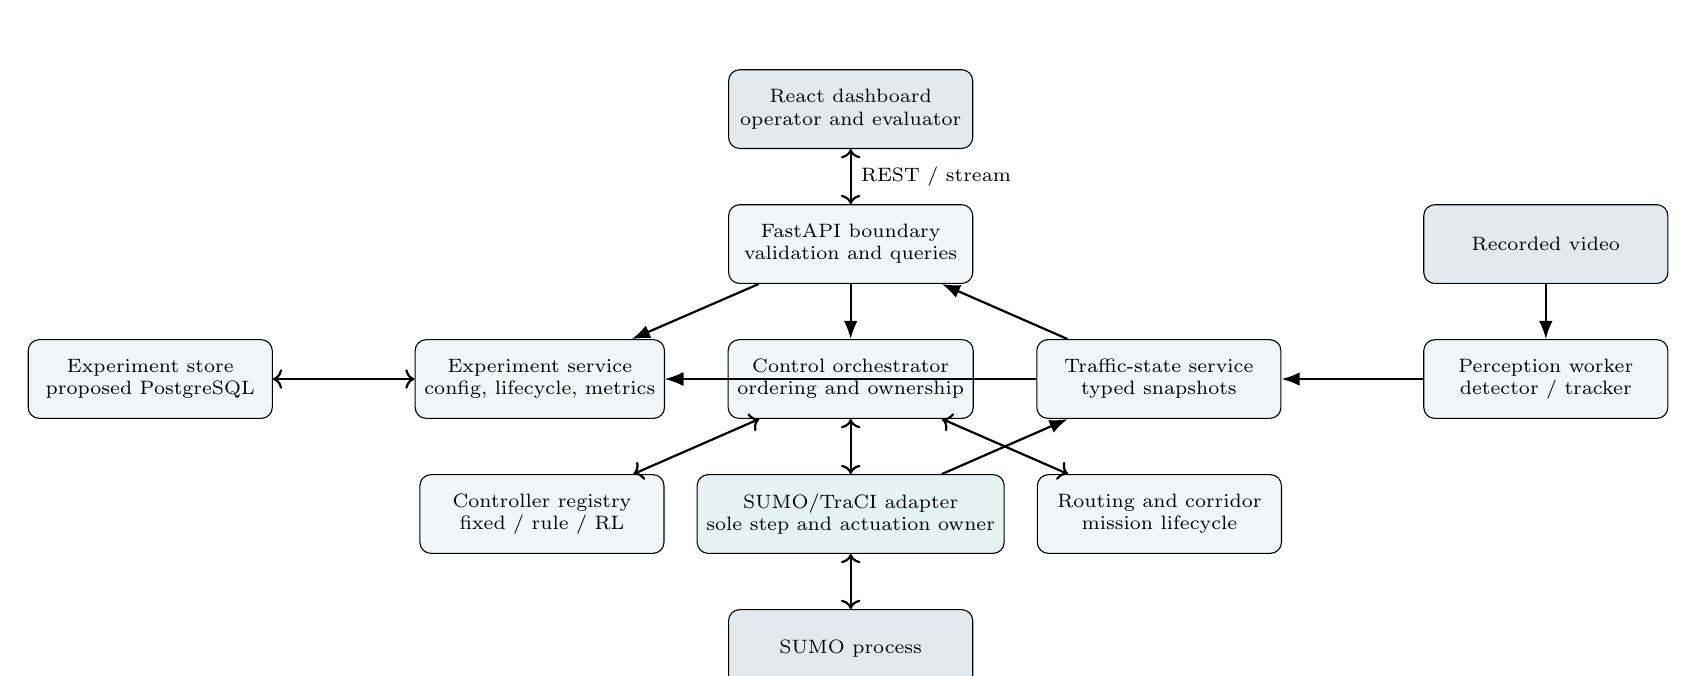
\begin{tikzpicture}[font=\scriptsize,node distance=7mm and 8mm,
comp/.style={draw,rounded corners,fill=manzilgray,minimum width=3.1cm,minimum height=1.0cm,align=center},
ext/.style={draw,rounded corners,fill=manzilblue!12,minimum width=3.1cm,minimum height=1cm,align=center},
arr/.style={-{Latex},thick}]
\node[ext] (ui) {React dashboard\\operator and evaluator};
\node[comp,below=of ui] (api) {FastAPI boundary\\validation and queries};
\node[comp,below left=of api] (exp) {Experiment service\\config, lifecycle, metrics};
\node[comp,below=of api] (orch) {Control orchestrator\\ordering and ownership};
\node[comp,below right=of api] (state) {Traffic-state service\\typed snapshots};
\node[comp,below left=of orch] (controller) {Controller registry\\fixed / rule / RL};
\node[comp,below=of orch,fill=manzilgreen!12] (sumoad) {SUMO/TraCI adapter\\sole step and actuation owner};
\node[comp,below right=of orch] (route) {Routing and corridor\\mission lifecycle};
\node[ext,below=of sumoad] (sumo) {SUMO process};
\node[comp,right=18mm of state] (per) {Perception worker\\detector / tracker};
\node[ext,above=of per] (video) {Recorded video};
\node[comp,left=18mm of exp] (store) {Experiment store\\proposed PostgreSQL};
\draw[arr,<->] (ui)--node[right]{REST / stream}(api);
\draw[arr] (api)--(exp);\draw[arr] (api)--(orch);\draw[arr] (state)--(api);
\draw[arr,<->] (orch)--(controller);\draw[arr,<->] (orch)--(route);\draw[arr,<->] (orch)--(sumoad);
\draw[arr,<->] (sumoad)--(sumo);\draw[arr] (sumoad)--(state);
\draw[arr] (video)--(per);\draw[arr] (per)--(state);
\draw[arr,<->] (exp)--(store);\draw[arr] (orch)--(exp);\draw[arr] (state)--(exp);
\end{tikzpicture}
}
\caption{Proposed high-level architecture}
\label{fig:architecture}
\end{figure}

The dashboard never calls TraCI. It sends validated commands to FastAPI and consumes views. The orchestrator executes Algorithm \ref{alg:loop}; the adapter alone advances SUMO and applies signals. Controllers return requests, not side effects. The routing and corridor service maintains mission/route versions and intersection priority states. The state service normalizes simulator or perception observations but preserves their source. The experiment service stores configuration and evidence.

\section{Component Responsibilities and Interfaces}

\begin{longtable}{p{0.23\textwidth}p{0.30\textwidth}p{0.36\textwidth}}
\caption{Component responsibility allocation}\label{tab:components}\\
\toprule
\textbf{Component} & \textbf{Consumes} & \textbf{Produces / owns}\\
\midrule\endfirsthead
\toprule
\textbf{Component} & \textbf{Consumes} & \textbf{Produces / owns}\\
\midrule\endhead
React dashboard & Query responses, event snapshots, user input & Presentation state; no control authority\\
FastAPI boundary & HTTP/stream commands, identity-free local operator session & Validation, command/query boundary, error mapping\\
Experiment service & Valid configuration, metric/event batches & Run lifecycle, immutable manifest, comparison eligibility\\
Control orchestrator & Run config and ordered state snapshot & Decision schedule, module ordering, requested actions\\
SUMO/TraCI adapter & Validated step and action commands & Simulation process, clock, subscriptions, applied actions\\
Traffic-state service & SUMO observations or perception messages & Versioned source-specific snapshots and freshness\\
Perception worker & Video and model configuration & Detections, tracks, aggregates, job health\\
Controller registry & State, legal phases, timing constraints & Requested normal-control action and explanation\\
Routing service & Graph, mission, cost snapshot & Route versions, no-route reason, reroute decision\\
Corridor coordinator & Route version, ambulance state, signal state & Priority request/state, release and recovery requests\\
Experiment store & Validated records and artifacts & Durable configuration, events, metrics, checksums\\
\bottomrule
\end{longtable}

\section{Architectural Decisions and Tradeoffs}

\begin{longtable}{p{0.20\textwidth}p{0.23\textwidth}p{0.23\textwidth}p{0.16\textwidth}}
\caption{Architectural decision record}\label{tab:decisions}\\
\toprule
\textbf{Decision} & \textbf{Selected approach} & \textbf{Alternative and reason not selected initially} & \textbf{Consequence}\\
\midrule\endfirsthead
\toprule
\textbf{Decision} & \textbf{Selected approach} & \textbf{Alternative and reason not selected initially} & \textbf{Consequence}\\
\midrule\endhead
Simulation ownership & One orchestrator/TraCI adapter controls stepping and signals & Multiple services calling TraCI risks non-deterministic order & Simple replay and concurrency model\\
Simulator & SUMO, as approved and supported by detailed road/signal tooling & CityFlow offers training throughput but changes the approved environment & Lower migration risk; performance profiled later\\
API/UI & FastAPI plus React, fixed by proposal & Server-rendered monolith would simplify deployment but reduce clear service contracts & Typed API and independent UI iteration\\
Controller integration & Common request interface plus safety filter & Direct controller access to TraCI couples research code to simulation & Comparable controllers; applied action may differ from request\\
Emergency control & Supervisory corridor state machine & Adding emergency reward directly to normal RL confounds attribution & Clear ablation and safety ownership\\
Routing & Dijkstra reference; A* only with admissible lower bound & Distance-only route is simpler but ignores the research question & Time-based, auditable costs\\
Persistence & Structured experiment schema; PostgreSQL proposed & Flat files are quick but weak for cross-run integrity & Engine remains replaceable behind repository interface\\
Perception execution & Background worker with bounded messages & In-request inference blocks API and control loop & Adds job state and queue management\\
\bottomrule
\end{longtable}

\section{Domain Model and Class Diagram}

\begin{figure}[H]
\centering
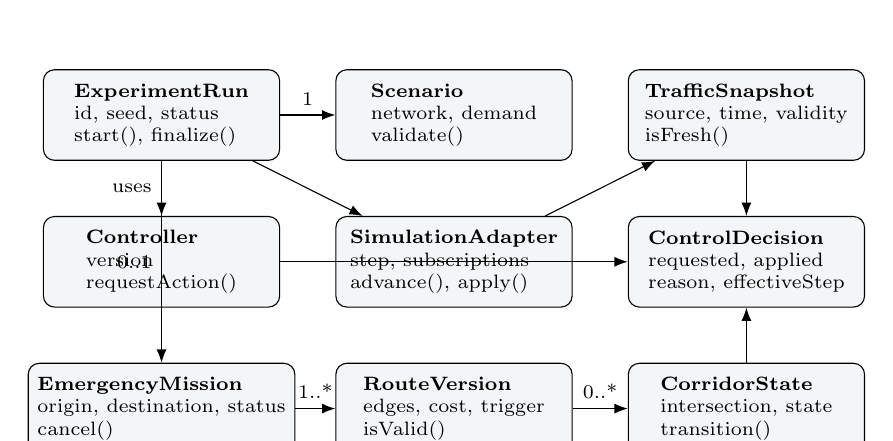
\begin{tikzpicture}[font=\scriptsize,node distance=7mm and 7mm,cls/.style={draw,rounded corners,fill=manzilgray,minimum width=3.0cm,minimum height=1.15cm,align=left},assoc/.style={-{Latex},thin}]
\node[cls] (run) {\textbf{ExperimentRun}\\id, seed, status\\start(), finalize()};
\node[cls,right=of run] (scenario) {\textbf{Scenario}\\network, demand\\validate()};
\node[cls,right=of scenario] (snap) {\textbf{TrafficSnapshot}\\source, time, validity\\isFresh()};
\node[cls,below=of run] (ctrl) {\textbf{Controller}\\version\\requestAction()};
\node[cls,below=of scenario] (adapter) {\textbf{SimulationAdapter}\\step, subscriptions\\advance(), apply()};
\node[cls,below=of snap] (decision) {\textbf{ControlDecision}\\requested, applied\\reason, effectiveStep};
\node[cls,below=of ctrl] (mission) {\textbf{EmergencyMission}\\origin, destination, status\\cancel()};
\node[cls,below=of adapter] (route) {\textbf{RouteVersion}\\edges, cost, trigger\\isValid()};
\node[cls,below=of decision] (corr) {\textbf{CorridorState}\\intersection, state\\transition()};
\draw[assoc] (run)--node[above]{1}(scenario);\draw[assoc] (run)--node[left]{uses}(ctrl);\draw[assoc] (run)--(adapter);\draw[assoc] (adapter)--(snap);\draw[assoc] (ctrl)--(decision);\draw[assoc] (snap)--(decision);
\draw[assoc] (run)--node[left]{0..1}(mission);\draw[assoc] (mission)--node[above]{1..*}(route);\draw[assoc] (route)--node[above]{0..*}(corr);\draw[assoc] (corr)--(decision);
\end{tikzpicture}
\caption{Proposed domain model/class diagram}
\label{fig:class}
\end{figure}

The domain model deliberately separates a requested decision from an applied decision. A controller can request an illegal early switch, but the safety filter and adapter determine the action actually applied. RouteVersion is immutable and corridor states refer to one version, allowing obsolete requests to be cancelled reliably.

\section{Interaction Sequences}

\subsection{Normal Control Update}

\begin{figure}[H]
\centering
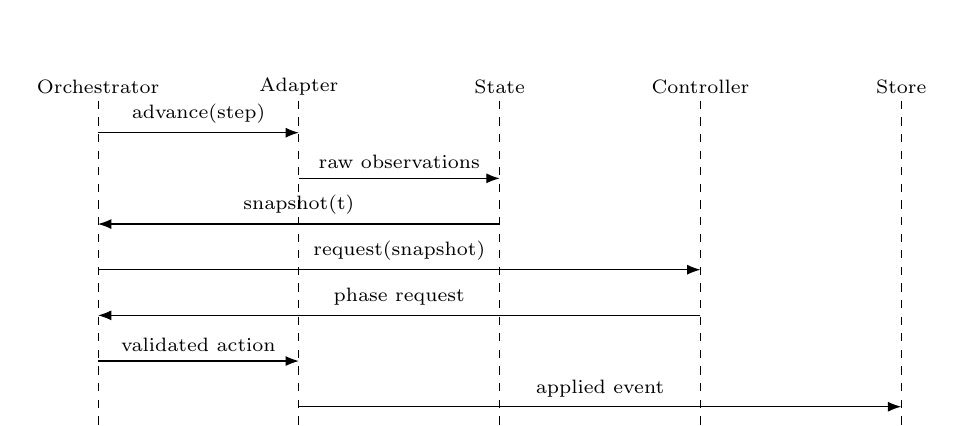
\begin{tikzpicture}[font=\scriptsize,x=2.55cm,y=.58cm]
\foreach \x/\n in {0/Orchestrator,1/Adapter,2/State,3/Controller,4/Store}{\node at (\x,0) {\n};\draw[dashed] (\x,-.3)--(\x,-7.7);}
\draw[-{Latex}] (0,-1)--node[above]{advance(step)}(1,-1);
\draw[-{Latex}] (1,-2)--node[above]{raw observations}(2,-2);
\draw[-{Latex}] (2,-3)--node[above]{snapshot(t)}(0,-3);
\draw[-{Latex}] (0,-4)--node[above]{request(snapshot)}(3,-4);
\draw[-{Latex}] (3,-5)--node[above]{phase request}(0,-5);
\draw[-{Latex}] (0,-6)--node[above]{validated action}(1,-6);
\draw[-{Latex}] (1,-7)--node[above]{applied event}(4,-7);
\end{tikzpicture}
\caption{Sequence for a normal signal-control update}
\label{fig:seq-normal}
\end{figure}

The snapshot is created only after the simulation step completes. A controller never observes a partial update. If a decision interval spans several simulation steps, the orchestrator reuses the last applied action while metrics continue to sample at their specified interval.

\subsection{Ambulance Dispatch and Corridor Activation}

\begin{figure}[H]
\centering
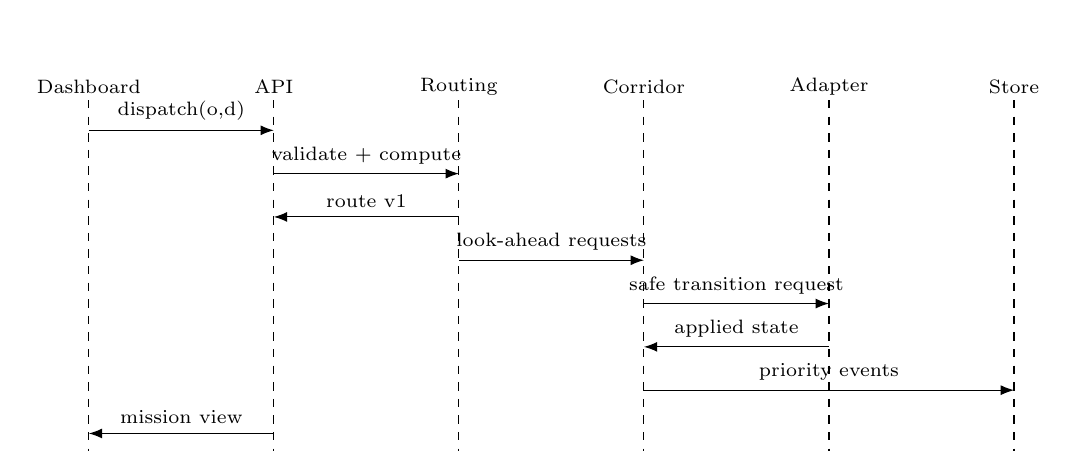
\begin{tikzpicture}[font=\scriptsize,x=2.35cm,y=.55cm]
\foreach \x/\n in {0/Dashboard,1/API,2/Routing,3/Corridor,4/Adapter,5/Store}{\node at (\x,0) {\n};\draw[dashed] (\x,-.3)--(\x,-8.7);}
\draw[-{Latex}] (0,-1)--node[above]{dispatch(o,d)}(1,-1);
\draw[-{Latex}] (1,-2)--node[above]{validate + compute}(2,-2);
\draw[-{Latex}] (2,-3)--node[above]{route v1}(1,-3);
\draw[-{Latex}] (2,-4)--node[above]{look-ahead requests}(3,-4);
\draw[-{Latex}] (3,-5)--node[above]{safe transition request}(4,-5);
\draw[-{Latex}] (4,-6)--node[above]{applied state}(3,-6);
\draw[-{Latex}] (3,-7)--node[above]{priority events}(5,-7);
\draw[-{Latex}] (1,-8)--node[above]{mission view}(0,-8);
\end{tikzpicture}
\caption{Sequence for ambulance dispatch and corridor activation}
\label{fig:seq-dispatch}
\end{figure}

\subsection{Rerouting and Recovery}

\begin{figure}[H]
\centering
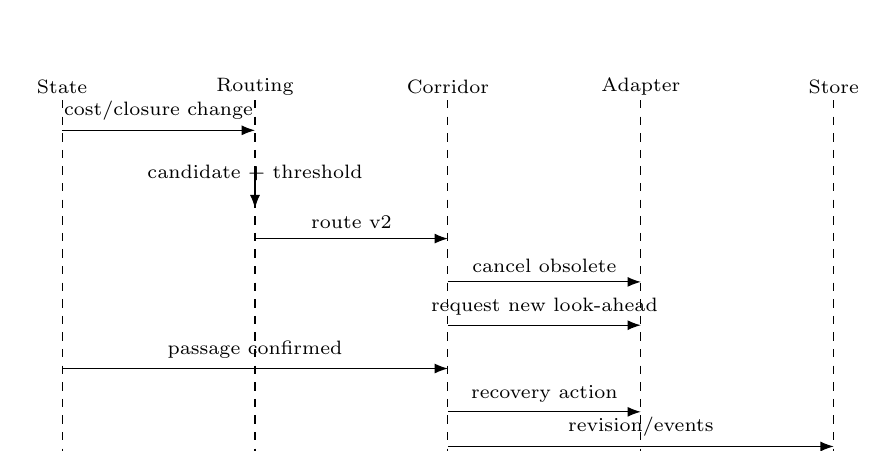
\begin{tikzpicture}[font=\scriptsize,x=2.45cm,y=.55cm]
\foreach \x/\n in {0/State,1/Routing,2/Corridor,3/Adapter,4/Store}{\node at (\x,0) {\n};\draw[dashed] (\x,-.3)--(\x,-8.7);}
\draw[-{Latex}] (0,-1)--node[above]{cost/closure change}(1,-1);
\draw[-{Latex}] (1,-2)--node[above]{candidate + threshold}(1,-2.8);
\draw[-{Latex}] (1,-3.5)--node[above]{route v2}(2,-3.5);
\draw[-{Latex}] (2,-4.5)--node[above]{cancel obsolete}(3,-4.5);
\draw[-{Latex}] (2,-5.5)--node[above]{request new look-ahead}(3,-5.5);
\draw[-{Latex}] (0,-6.5)--node[above]{passage confirmed}(2,-6.5);
\draw[-{Latex}] (2,-7.5)--node[above]{recovery action}(3,-7.5);
\draw[-{Latex}] (2,-8.3)--node[above]{revision/events}(4,-8.3);
\end{tikzpicture}
\caption{Sequence for route revision, obsolete-priority cancellation, and recovery}
\label{fig:seq-reroute}
\end{figure}

\section{Corridor State Model}
\label{sec:corridor-state}

\begin{figure}[H]
\centering
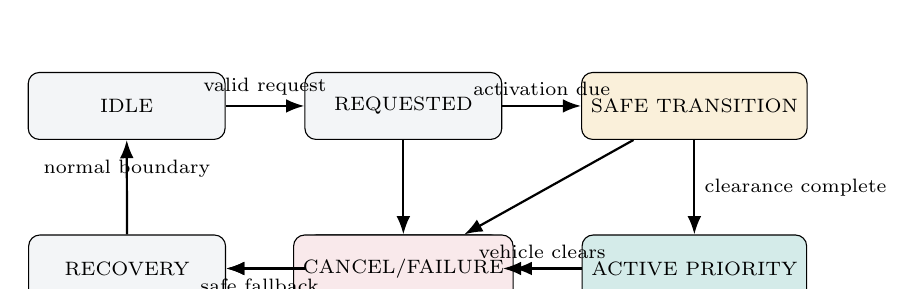
\begin{tikzpicture}[font=\scriptsize,node distance=12mm and 10mm,st/.style={draw,rounded corners,minimum width=2.5cm,minimum height=.85cm,align=center,fill=manzilgray},arr/.style={-{Latex},thick}]
\node[st] (idle) {IDLE};
\node[st,right=of idle] (req) {REQUESTED};
\node[st,right=of req,fill=manzilamber!25] (trans) {SAFE TRANSITION};
\node[st,below=of trans,fill=manzilgreen!20] (active) {ACTIVE PRIORITY};
\node[st,left=of active] (passed) {PASSAGE};
\node[st,left=of passed] (recover) {RECOVERY};
\node[st,below=of req,fill=manzilred!12] (cancel) {CANCEL/FAILURE};
\draw[arr] (idle)--node[above]{valid request}(req);
\draw[arr] (req)--node[above]{activation due}(trans);
\draw[arr] (trans)--node[right]{clearance complete}(active);
\draw[arr] (active)--node[above]{vehicle clears}(passed);
\draw[arr] (passed)--(recover);\draw[arr] (recover)--node[above]{normal boundary}(idle);
\draw[arr] (req)--(cancel);\draw[arr] (trans)--(cancel);\draw[arr] (active)--(cancel);
\draw[arr] (cancel)--node[below]{safe fallback}(recover);
\end{tikzpicture}
\caption{Intersection-level moving-corridor state transitions}
\label{fig:corridor-state}
\end{figure}

State transitions are event-driven and guarded. REQUESTED does not imply signal ownership. SAFE TRANSITION waits for the normal phase's minimum service and clearance. ACTIVE PRIORITY has a maximum duration. PASSAGE is a recorded event, and RECOVERY must complete before the normal controller resumes direct ownership. Cancellation never jumps directly to an arbitrary normal phase.

\section{Traffic-State and Event Contracts}

\begin{longtable}{p{0.20\textwidth}p{0.21\textwidth}p{0.46\textwidth}}
\caption{Core interface and data-contract fields}\label{tab:contracts}\\
\toprule
\textbf{Contract} & \textbf{Required fields} & \textbf{Rule}\\
\midrule\endfirsthead
\toprule
\textbf{Contract} & \textbf{Required fields} & \textbf{Rule}\\
\midrule\endhead
TrafficSnapshot & schemaVersion, sourceMode, producedAt, effectiveStep, validUntil, networkId & Consumers reject unknown schema or expired validity; wall time and simulation time are distinct.\\
ApproachState & intersectionId, approachId, count, queue, wait, speed, occupancy, units, confidence & Missing is not zero; uncalibrated physical quantities are omitted.\\
SignalState & intersectionId, programId, phaseId, phaseElapsed, legalNext, owner & Owner is NORMAL or CORRIDOR; legal next phases come from validated configuration.\\
ControlRequest & controllerId, intersectionId, requestedPhase, duration/extension, snapshotStep, reason & Request has no side effect and may be rejected or transformed.\\
AppliedControl & requestId, appliedPhase, effectiveStep, safetyIntervention, reason & This record is authoritative for analysis.\\
RoutePlan & missionId, routeVersion, edgeIds, costSeconds, snapshotStep, trigger & Edge order must be continuous from valid current position.\\
PriorityRequest & missionId, routeVersion, intersectionId, movementId, ETA, expiresAt & Obsolete route version or expired request is rejected.\\
MetricSample & runId, metricName, metricVersion, interval, value, unit & Aggregation across mismatched versions is prohibited.\\
\bottomrule
\end{longtable}

Event ordering is based on simulation step within a run and a monotonic sequence number assigned by the orchestrator. Wall-clock timestamps support diagnostics but do not determine traffic causality. Route revisions and priority events are committed in an order that prevents an old request from being interpreted as current.

\section{Concurrency, Synchronization, and Resource Ownership}

The orchestrator is the only writer to simulation time. TraCI access is serialized behind the adapter. Controller computation receives an immutable snapshot. Perception uses a bounded work queue; if it falls behind, the worker marks observations late rather than blocking control. Dashboard streams are lossy views: a slow client may skip intermediate snapshots but cannot delay decisions.

Run configuration is immutable after start. The current route version is updated atomically with the cancellation of obsolete corridor requests. Database writes are batched where safe, but an applied signal event and mission-state transition must not be acknowledged before durable enqueue. On shutdown, the system stops accepting commands, terminates or detaches SUMO safely, flushes records, and gives the run an explicit terminal state.

\section{Error Handling and Fallback}

\begin{table}[H]
\centering
\caption{Failure handling strategy}
\label{tab:errors}
\begin{tabularx}{\textwidth}{p{0.27\textwidth}YY}
\toprule
\textbf{Failure} & \textbf{Immediate behavior} & \textbf{Recorded/recovery behavior}\\
\midrule
SUMO launch/TraCI disconnect & Stop decisions and do not present live state & Mark run failed; retain command, stderr, step, and manifest\\
Stale observation & Exclude or use declared simulator fallback & Record staleness and selected fallback source\\
Invalid controller action & Reject through safety filter & Apply fixed/safe continuation and record intervention\\
RL service unavailable & Switch at valid boundary to configured baseline & Record fallback interval; exclude from clean RL aggregate or report separately\\
No route & Do not spawn/activate partial corridor & Mark mission blocked; show cause and graph snapshot ID\\
Lost ambulance/timeout & Cancel future priority and recover active intersections & Mark mission failed/cancelled and preserve last position\\
Persistence failure & Buffer within a bounded queue; stop before unbounded evidence loss & Mark run incomplete if durability cannot be restored\\
Dashboard disconnect & Continue experiment unaffected & Reconnect from current snapshot and event cursor\\
\bottomrule
\end{tabularx}
\end{table}

\section{Detailed Module Policies}

\subsection{Controller Policy}

All controllers implement a common method accepting a snapshot, intersection configuration, and decision context, and returning a request plus explanation fields. They cannot write global state or call TraCI. Deterministic evaluation disables exploration and seeds all permitted stochastic operations. The safety filter verifies phase membership, minimum green, clearance, maximum priority duration, and ownership.

\subsection{Routing Policy}

The graph builder derives edges from validated SUMO movements. Cost providers are composable but must state units and whether link time already includes queue delay. A route plan is immutable. The mission points to one current version, and a revision is accepted only through Algorithm \ref{alg:routing}. Closures override cost and invalidate affected routes immediately.

\subsection{Persistence Policy}

The store uses migrations and foreign keys for structured data, and checksummed external artifacts for large files. Raw high-frequency state may be downsampled for persistence, but the interval and aggregation method are recorded. Secrets or local filesystem paths are not exported as research data. Database selection will be confirmed by implementation; the domain schema is independent of that choice.

\subsection{User-Interface Policy}

Colors are supplemented with labels and icons so congestion or failures are not conveyed by color alone. Units and source mode appear beside values. Schematic predictions and measured values are visually distinct. The UI does not display ``time saved'' until a valid reference run exists under the same comparison manifest.

\section{Testing Strategy}

Unit tests cover cost functions, route validity, hysteresis, metric calculations, schema validation, and corridor transition guards. Property or invariant tests generate action sequences to ensure incompatible greens are never produced and that corridor cancellation eventually reaches IDLE through RECOVERY. Integration tests run small SUMO networks to validate step ownership, detector-to-state messages, route application, and persistence. Scenario tests replay fixed seeds for normal control, closure rerouting, no-route, controller failure, stale data, ambulance timeout, and dashboard disconnect.

Research verification is separate from software correctness. Passing unit tests shows that the implementation follows its specification; it does not show that the policy improves traffic. Comparative experiments described in Chapter \ref{ch:method} provide that evidence.

\section{Coding, Build, and Maintainability Policies}

Python modules will use static type hints, formatting and linting, bounded dependency versions, structured logging, and docstrings for public interfaces. React components will separate data fetching from presentation. Configuration is stored as validated files rather than scattered constants. Continuous checks should run unit tests and a minimal headless SUMO scenario. Releases used for experiments are tagged and their commit ID is written into run manifests.

The intended repository structure separates application services, controllers, routing, perception, simulation, dashboard, schemas, scenarios, and experiment artifacts. This is a proposed organization, not evidence that those directories already exist. Small interfaces allow a tracker, RL algorithm, database, or dashboard transport to change without rewriting the simulation loop.

\section{Conclusion}

The design assigns one clear owner to every mutable resource and makes source, time, units, route version, and applied action explicit. The architecture supports the intended progression from baselines to RL and from static routing to a safe moving corridor, while allowing failures and negative experimental outcomes to be recorded honestly. It is sufficiently modular for team implementation without requiring distributed-system complexity at the prototype stage.


\cleardoublepage
\bibliographystyle{ieeetr}
\bibliography{references}

\appendix
\chapter{Deliverable 2 Requirements Coverage}
\label{app:coverage}
\begin{longtable}{p{0.27\textwidth}p{0.29\textwidth}p{0.35\textwidth}}
\caption{Requirements coverage matrix}\label{tab:coverage}\\
\toprule
\textbf{Deliverable requirement} & \textbf{Primary evidence} & \textbf{Report location}\\
\midrule\endfirsthead
\toprule
\textbf{Deliverable requirement} & \textbf{Primary evidence} & \textbf{Report location}\\
\midrule\endhead
Project purpose and vision & Approved proposal and maintained context & Chapters 1--2\\
At least 15 relevant studies & Verified peer-reviewed literature and official papers & Chapter 3 and bibliography\\
Software requirements and use cases & Proposal scope and planned operator workflow & Chapter 4\\
GUI and data design & Proposed dashboard and persistence needs & Sections \ref{sec:gui}--\ref{sec:data-design}\\
Research methodology & Proposal baselines and reproducible evaluation plan & Chapter 5\\
High- and low-level design & Service responsibilities and control safety constraints & Chapter 6\\
Architecture, UML, sequences, state model & Original TikZ diagrams & Sections \ref{sec:architecture}--\ref{sec:corridor-state}\\
Honest project status & Proposal stage statement and repository evidence & Throughout; Section \ref{sec:status}\\
\bottomrule
\end{longtable}

\chapter{Open Items for Team Confirmation}
\label{app:open-items}
The report remains usable without resolving the items below, but they must be confirmed before an implementation or final-results report makes corresponding claims.
\begin{enumerate}
  \item Exact Lahore road area, network size, and imported OpenStreetMap snapshot.
  \item Final detector checkpoint, tracker configuration, annotated video sources, and license records.
  \item Final RL algorithm and hyperparameters after baseline feasibility tests.
  \item Database selection, demonstration hardware, and measured update/latency targets.
  \item Actual application screenshots, once the interfaces exist; all current interface figures are labelled as proposed wireframes.
  \item Any faculty-issued certificate or approval page not present in the supplied FAST template.
\end{enumerate}

\end{document}
